 \documentclass[
 ]{scrarticle}
\typeout{****** X0}
% TODO: Wording im ganzen Dokument vereinheitlichen: Instanz/instanziieren statt Projektion/projizieren.
\usepackage{osgdoc}
\typeout{*************** X0A}
%\usepackage{xcolor}
\usepackage{hyperref}
\typeout{****** X1}
\usepackage{enumitem}
\usepackage{fontspec}
\typeout{****** X2}
\usepackage{microtype}
\usepackage{dirtreex}
\usepackage{tcolorbox}
\typeout{****** LOAD LANGSELECT}
\usepackage[
languages={de,en},
map={de=german,en=english},
targetlang={job=3},
load babel
]{langselect}
\usepackage{hologo}
\usepackage{subcaption}

\colorlet{linkblue}{blue!50!black}
\newcommand{\osglecture}{\textcolor{blue}{OSG Lecture}}

\hypersetup{
  pdftitle  = {OSG Lecture Bundle - Benutzerhandbuch},
  pdfauthor = {Matthias Werner},
  colorlinks,
  linkcolor = linkblue,
  urlcolor  = linkblue
}
\author{Matthias Werner}
\title{\ldeen{Das OSG Lecture Bundle}{}}
\subtitle{\ldeen{Benutzerhandbuch}{User Manual}}
\KOMAoptions{parskip=half,toc=indented}

\begin{document}
\maketitle

\begingroup
\parskip=2pt
\tableofcontents
\endgroup
\captionsetup{font=footnotesize,labelfont=bf,textfont=sf,skip=2pt}

\section{\ldeen{Einführung}{Introduction}}
\subsection{\ldeen{Idee}{Idea}}
\ldeen{Lehrmaterialien treten in vielerlei Formen und Versionen auf, beispielsweise als
  Vorlesungsskript, Folien oder Handouts, und das möglicherweise jeweils in verschiedenen Sprachen.
  Dabei sind die Inhalte oft gleich oder ähnlich, und die Stukturen~-- beispielsweise die
  Reihenfolge der Lehr- und Lerneinheiten sollten konsistent sein.}{
  Teaching materials come in many forms and versions, such as
  lecture notes, slides, or handouts, and may be available in different languages.
  Yet the content is often the same or similar, and the structures—for example, the
  order of the teaching and learning units—should be consistent.
}
\ldeen*{Mit anderen Worten: Die gleiche Sache (hier: semantische Information) soll in unterschiedlicher Gestalt auftreten. In der Informatik oder in der Chemie nennt man dieses Konzept auch \emph{Polymorphie}@1.}{
  In other words: The same thing (here semantic information) should appear in different forms.
In computer science or chemistry, this concept is also known as \emph{polymorphism}@1
}{\footnote{\ldeen{
  Vielleicht wären \emph{Polyrepräsentation} oder sogar \emph{Multimodalität} noch passendere Begriffe,
  aber ersteres ist nicht sehr etabliert und beim zweiteren müsste ich vermutlich mit Kulturwissenschaftlern und Semiotikern darüber diskutieren, ob unterschiedliche Sprachen als \emph{Modi} aufzufassen sind.
  Außerdem bin ich Informatiker, da liegt die Polymorphie nahe.
  }{
    Perhaps \emph{poly-representation} or even \emph{multimodality} would be even more appropriate terms,
  but the former isn’t very well established, and with the latter, I’d probably have to discuss with cultural studies scholars and semioticians whether different languages should be understood as \emph{modes}.
  Besides, I’m a computer scientist, so polymorphism seems like a natural choice.}
}}

\ldeen{
  Gleichzeitig werden Lehrmaterialien in der Regel permanent überarbeitet. Einzelne Lehreinheiten
  werden modernisiert, reorganisiert oder gleich ganz entfernt, neue werden ergänzt.
}{
  At the same time, teaching materials are generally revised on an ongoing basis.
  Individual teaching units are updated, reorganized, or removed entirely, while new ones
  are added.
}
\ldeen*{
  Dabei stets die gewünschte Konsistenz aufrechtzuerhalten, ist schwierig. Das @1 Bundle
  versucht, Lehrende dabei zu unterstützen. Es folgt dabei einer zentralen Idee:
}{
  Maintaining the desired consistency throughout this process is difficult. The @1 Bundle
  aims to support instructors in this effort. It is based on a central idea:
}{\osglecture}
\footnote{
  \ldeen*{Es ist mir durchaus bewusst, dass dieser Leitgedanke nicht allgemein geteilt wird:
  ein \LaTeX-Riese wie \name{Joseph Wright} steht dieser Idee z.\,B. skeptisch gegenüber (@2),
  und er kann gute Gründe anbringen. Falls Sie also glauben, dass solche Gründe überwiegen, nutzen Sie @1 nicht.}{I am well aware that not everyone shares this guiding principle;
  a \LaTeX giant like \name{Joseph Wright}, for example, is skeptical of this idea (@2),
  and he can cite good reasons for his skepticism. So if you believe that such reasons outweigh the benefits, do not use @1.}
  {\osglecture}
  {\url{https://github.com/josephwright/ltx-talk/discussions/68\#discussioncomment-13755453}}
}
\begin{infobox}{\ldeen{Leitsatz}{Maxim}}\sffamily
\ldeen{Es sollten so \textbf{wenig} wie möglich \textbf{Redundanzen} auftreten.
  }{
    \textbf{Redundancies} should be kept to a \textbf{minimum}.
  }\medskip

  \ldeen{Wo Redundanzen notwendig sind (beispielsweise bei verschiedenen Textversionen),
  ist die Aufrechterhaltung von Konsistenz einfacher, wenn aufeinander
  bezogenes Quellmaterial \textbf{möglichst nahe} beieinander ist.
  }{
    Where redundancies are necessary (for example, with different versions of a text),
    it is easier to maintain consistency if related
    source material is located as \textbf{close together} as possible.}
\end{infobox}


\ldeen*{Daher soll @1 u.\,a.{} ermöglichen
}{
  Therefore, @1 is intended, amongst other things, to enable}{\osglecture}:
\begin{itemize}
  \item \ldeen{Generierung verschiedener Dokumentarten aus der gleichen Quelle
  }{
    Generating different types of documents from the same source
  };
  \item \ldeen{einfache Reorganisation von Lehreinheiten}{easy reorganization of teaching units};
  \item \ldeen{verschiedene Sprachvarianten aus der gleichen Quelle,
        wobei gemeinsame Daten nicht redundant dargestellt werden brauchen}{
        different language versions from the same source,
        wherein shared data does not need to be presented redundantly};
  \item \ldeen{Unterstützung bei individuellen Erstellen und Überarbeiten von
        Lehreinheiten mit einfacher Integration (z.\,B.{} Skriptkapitel zu einem
        Gesamtskript)}{
        support for creating and revising individual
        instructional units that can be easily integrated (e.g., lecture notes chapters into a
        comprehensive set of lecture notes)
        };
  \item \ldeen{schnelle Bereitstellung der verschiedenen Dokumentarten
  }{
    rapid deployment of the various types of document}.
\end{itemize}

\ldeen*{Dabei wurde von Modalitäten und Arbeitsabläufen ausgegangen, die
  an der Professur für Betriebssysteme (\emph{Operating Systems Group, OSG})
  der TU Chemnitz derzeit üblich sind.
  Wenn Sie nicht dort tätig sind und völlig andere Abläufe haben, könnte
  @1 trotzdem für Sie nützlich sein: einzelne Pakete des Bundles lassen sich
  auch unabhängig von den anderen nutzen.
  }{
    This was based on the procedures and workflows that
    are currently standard practice at the Operating Systems Group at Chemnitz University of Technology.
    If you do not work there and, for example, have different procedures,
    @1 might still be useful to you: individual packages within the bundle can
    also be used independently of the others.
  }{\osglecture}

\ldeen*{@1 ist das Nachfolgeprojekt von @2, das sich aus einem
  Thema und einer handvoll Ergänzungsmacros für die überaus verbreitete Beamer-Klasse@3
  entwickelt hat.
  Gegenüber seinem Vorgänger zeichnet sich @1 durch einen größeren Funktionsumfang,
  ein überarbeitetes und damit hoffentlich besseres Interface, eine umfangreichere
  Dokumentation und nicht zuletzt dadurch aus, dass es ermöglicht, barrierefreie getaggte
  Lehrdokumente zu erstellen, indem es Klassen wie \cls{ltx-talk} unterstützt.
  }{@1 is the successor project to @2, which has evolved from a
  theme and a handful of supplementary macros for the widely used Beamer class@3.
  }
  {\osglecture}
{\textcolor{teal!50!black}{OSG Beamer}\footnote{\url{https://github.com/tuc-osg/osgbeamer}}}
{\footnote{\url{https://ctan.org/pkg/beamer}}}

\subsection{\ldeen{Was genau \emph{ist} denn nun \osglecture?}{So what exactly \emph{is} \osglecture?}}
\ldeen{\osglecture{} ist ein \LaTeX-Bundle (genauer gesagt: ein \LuaLaTeX-Bundle), das verschiedene Ideen und Ansätze zusammenbringt um Lehrmaterialien zu erstellen. Keine dieser Ideen oder Ansätze ist besonders neu.
}{\osglecture{} is a \LaTeX bundle (more specifically, a \LuaLaTeX bundle) that brings together various ideas and approaches for creating teaching materials. None of these ideas or approaches is particularly new.}

\begin{itemize}
  \item \ldeen{
    \cls{osglecture} ist eine Metaklasse, die die meiste Arbeit an andere Klassen deligiert, so wie es z.\,B.{} auch \needpackage{beamerswitch} macht. Darüber hinaus stellt \cls{osglecture} aber
    auch einige Dinge selbst bereit, wie ein dokumentübergreifenden Referenzsystem und sogar einige 
    Fromatierungsumgebungen.
  }{
    \cls{osglecture} is a metaclass that delegates most of the work to other classes, much like 
    \needpackage{beamerswitch}, for example. In addition, \cls{osglecture} itself provides several features,
    including a cross-document reference system and even some formatting environments.}
  \item \ldeen{
    \pkg{langselect} ist ein Paket, das zur (sprachabhängigen) Auswahl von in das Ziel-PDF zu übernehmenden
    Text, ähnlich wie es auch \needpackage{comment} oder \needpackage{multilang} macht. 
    Die tatsächliche genutzte Sprache kann auch von außen festgelegt werden.
  }{
    \pkg{langselect} is a package for selecting which text is to be included in the target PDF depending on the 
    language, similar to \needpackage{comment} or \needpackage{multilang}. The language actually used can also 
    be specified externally.}
  \item \ldeen{
    \pkg{osglecture-modes} generalisiert die Idee von Darstellungsmodi, wie man sie aus \needpackage{beamer} 
    oder \needpackage{ltx-talk} kennt, macht also etwas ähnliches wie \pkg{langselect}, aber nicht auf
    Sprach- sondern auf Strukturebene. Damit können Modi in der aus \pkg{Peamer} oder \pkg{ltx-talk} 
    gewohnten \texttt{<>}-Syntay auch außerhalb von Präsentationen genutzt werden.
  }{
    \pkg{osglecture-modes} generalizes the concept of presentation modes familiar from \needpackage{beamer} 
    or \needpackage{ltx-talk}. It therefore does something similar to \pkg{langselect}, but at the structural 
    rather than the language level. This makes it possible to use modes outside presentations, too, with the 
    familiar \texttt{<>} syntax of \pkg{beamer} or \pkg{ltx-talk}.}
  \item \ldeen{
    \pkg{tagpax} dient dazu, getaggte PDF-Dokumente zu einem wiederum getaggten PDF-Dokument zu vereinen. 
    Es hat lange nicht soviel Möglichkeiten wie \needpackage{pdfpages} und baut auf den Ideen von 
    \needpackage{pax}/\needpackage{newpax} auf, behält aber nicht nur Annotationen sondern auch die 
    Taggingstruktur bei. Im Kontext von \osglecture{} dient es dazu, unabhängige Übersetzungen 
    z.\,B.\ einzelner Skriptkapitel zu einem Gesamtskript zu ermöglichen, ohne einen "`großen"' 
    Übersetzungslauf\footnote{Bei meinem Lehrskripten kann so ein großer Lauf durchaus auch mal über 
    eine Stunde dauern.} durchführen zu müssen.
  }{
    \pkg{tagpax} combines tagged PDF documents into a PDF document that is itself tagged. It provides far
    fewer features than \needpackage{pdfpages} and builds on the ideas of \needpackage{pax}/\needpackage{newpax}, 
    but preserves not only annotations, but also the tagging structure. In the context of \osglecture{}, it makes 
    it possible to compile, for example, individual lecture notes chapters independently and combine them into 
    a complete set of lecture notes without having to perform one "`large"' compilation run.\footnote{For my lecture
    notes, such a large run can sometimes take more than an hour.}
    }
  \item \ldeen{
    \OLLM{} ist ein \emph{yet another} Build-Tool, aber speziell auf \osglecture{} zugeschnitten und
    arbeitet eng mit \cls{osglecture} und den anderen genannten Paketen zusammen. Intern ruft \OLLM{} intern 
    \File{latexmk} auf (es ist aus einem rc-File für \File{latexmk} entstanden), das die meiste Arbeit erledigt.
  }{
    The \OLLM{} is a yet another build tool that is tailored specifically to \osglecture{} and works closely with 
    \cls{osglecture} and the other packages mentioned above. Internally, \OLLM{} invokes \File{latexmk}--it
    originated as an rc file for \File{latexmk}--which performs most of the work.}
\end{itemize}

\ldeen{Während diese genannten Pakete den Kern des Bundles bilden, gibt es noch einige Pakete, die sich 
  für die Erstellung von Lehrmaterialien als nützlich erwiesen haben. Diese interagieren durchaus mit den 
  Kernpaketen, tragen aber mehr zur direkten Gestaltung der Dokumente bei, als zur Realisierung des 
  Polymorphieansatzes, den sie aber nutzen.
}{While the packages mentioned above form the core of the bundle, several additional packages have proved 
  useful for creating teaching materials. They do interact with the core packages, but contribute more directly
  to the design of the documents than to implementing the polymorphism approach, although they make use of it.}
\begin{itemize}
  \item \ldeen{\pkg{osgstyler} versucht die \LaTeX-Kernidee der Trennung von Inhalt und Gestaltung
    über eine zentrale semantische Konfiguration zu stärken. Dinge wie Farben, Schriften, Abstände, Hervorhebungen
    und Blöcke können damit einerseits einfacher konsistent und andererseits leichter austauschbar gestaltet werden.
    Es kann gut mit \pkg{osglecture-modes} zusammenwirken.
  }{\pkg{osgstyler} seeks to reinforce the core \LaTeX{} principle of separating content from presentation 
    through a central semantic configuration. This makes elements such as colors, fonts, spacing, highlighting, 
    and blocks easier to design consistently as well as easier to replace. It works well in conjunction with \pkg{osglecture-modes}.}
  \item \ldeen{\pkg{ltxtalk-theme} ist eine experimentelle Theme-Engine für \cls{ltx-talk}. Für "`innere"'
    Gestaltungsaspekte wird \pkg{osgstyler} genutzt. Vermutlich wird \pkg{ltxtalk-theme} mit der weiteren Entwicklung
    von \cls{ltx-talk} irgendwann überflüssig.}{\pkg{ltxtalk-theme} is an experimental theme engine for 
    \cls{ltx-talk}. It uses \pkg{osgstyler} for inner design aspects. As \cls{ltx-talk} continues to evolve, 
    \pkg{ltxtalk-theme} will probably become obsolete eventually.}
  \item \ldeen{\pkg{lttheme-tuc-2019} ist die (inoffizielle) Umsetzung des offiziellen Präsentationslayout meiner
    Universität für \pkg{ltx-talk}. Es nutzt \pkg{ltxtalk-theme}.
  }{\pkg{lttheme-tuc-2019} is the unofficial implementation of my university's official presentation layout 
    for \pkg{ltx-talk}. It uses \pkg{ltxtalk-theme}.}
  \item \ldeen{\pkg{semcat} dient zur einfacheren semantischen Markierung (z.\,B.\ von Kategorien wie
    "`Hintergründe"',  "`technische Details"' oder "`Wiederholung"') von Textteilen oder QR-Codes.
  }{\pkg{semcat} facilitates the semantic labeling of passages of text or QR codes, for example with categories 
    such as "`background"', "`technical details"', or "`review"'.}
  \item \ldeen{\pkg{ansiterm} stellt zwei semiverbatim Umgebungen für die Darstellung von Computerterminalfenstern zur
    Verfügung, die ANSI-Escapesequenz\footnote{Siehe z.\,B.\ \url{https://de.wikipedia.org/wiki/ANSI-Escapesequenz}}
    interpretieren können. Eine davon führt zur Übersetzungszeit den Inhalt in einer Shell aus und liest die
    Ergebnisse zurück, simuliert also ein "`echtes"' Terminal.
  }{\pkg{ansiterm} provides two semiverbatim environments for displaying computer terminal windows that can 
    interpret ANSI escape sequences\footnote{See, for example, \url{https://en.wikipedia.org/wiki/ANSI_escape_code}.}. 
    One of them executes its contents in a shell at compilation time and reads back the results, thus simulating a 
    "`real"' terminal.}
  \item \ldeen{\pkg{osglistings} stellt ein Frontend für \needpackage{minted} zur Verfügung mit erweiterten 
    Möglichkeiten der Quellcodemarkierung, Einbindung von Gists und Repositories und verschiedenen Darstellungen.
  }{\pkg{osglistings} provides a front end for \needpackage{minted}, offering advanced source-code highlighting, the 
    inclusion of gists and repositories, and various presentation styles.}
\end{itemize}

\subsection{\ldeen{Polymorphie}{Polymorphism} in \osglecture}
\ldeen{Es ist eine alte \hologo{TeX}-Idee, Texte je nach Kontext unterschiedlich darzustellen. Die \hologo{TeX}-Variante \hologo{ConTeXt} leitet beispielsweise ihren Namen auch davon ab.
\osglecture{} versucht die Anwendung dieses Konzept noch ein Stück weit zu erweitern.
Dazu ist \cls{osglecture} eine \emph{Metaklasse}: Sie sagt (anders als die meisten
\LaTeX-Klassen) nicht, wie die fertig gesetzten Dokumente aussehen sollen,\footnote{Es gibt aber
Pakete im \osglecture-Bundle, die so etwas machen} sondern stellt ein gemeinsames Interfache zur
Verfügung und verteilt dann die Arbeit an Klassen wie \cls{article}, \cls{scrarticle}, \cls{beamer}
oder \cls{ltx-talk}.}{It is a
long-standing \hologo{TeX} concept to render text differently depending on the
context. The \hologo{TeX} variant \hologo{ConTeXt}, for example, derives its
name from this concept. \osglecture{} attempts to expand the application of this concept a bit further.
In this regard, \cls{osglecture} is a \emph{metaclass}: Unlike most
\LaTeX{} classes, it does not specify how the final typeset documents should look,\footnote{However, there are
packages in the \osglecture bundle that do just that} but rather provides a common interface
and then delegates the work to classes such as \cls{article}, \cls{scrarticle}, \cls{beamer},
or \cls{ltx-talk}.}

\ldeen{Das Folgende ist ein Mini-Showcase der zeigen soll, wie aus einer Quelle verschiedene Instanzen
erzeugt werden. Es dient lediglich dazu, dass der Nutzer einen kleinen Eindruck von den
Möglichkeiten des kontextabhängigen Polymorphismus in \osglecture{} gewinnen kann~-- die Diskussion
über Funktionsweise und die verwendeten Mechanismen erfolgt später.}{
The following is a mini-showcase designed to demonstrate how different instances are
created from a single source. Its sole purpose is to give the user a brief glimpse of the
possibilities of context-dependent polymorphism in \osglecture{}-—the discussion
of how it works and the mechanisms used will follow later.}

%\begin{figure}[h]
\begin{minipage}{\linewidth}
  \inputsourcecode[
    gobble=0,
    add-local-frame={innerleftmargin=12pt,innerrightmargin=8pt},
    add-sourcecode-options={breaklines=true,breakatwhitespace=true,
    columns=fullflexible,basicstyle=\footnotesize}
  ]{polymorphy-source.tex}
  \captionof{figure}{\label{fig:common-src}\ldeen{Gemeinsamer Quellcode}{Common source code}}
\end{minipage}

\begin{minipage}{\linewidth}
  \captionsetup{type=figure}
  \centering
  \begin{subcaptiongroup}
    \begin{minipage}[t]{.48\linewidth}
      \fbox{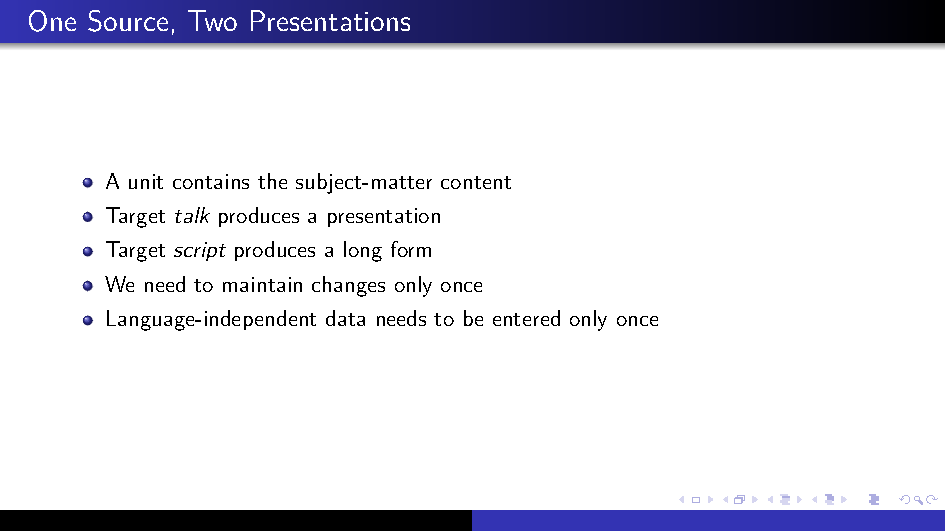
\includegraphics[page=1,width=\linewidth]{polymorphy-slides-en.pdf}}
      \caption{\ldeen{Folien auf English}{Slides in English}}
    \end{minipage}\hfill
    \begin{minipage}[t]{.48\linewidth}
      \fbox{\includegraphics[page=1,width=\linewidth]{polymorphy-slides-de.pdf}}
      \caption{\ldeen{Folien auf Deutsch}{Slides in German}}
    \end{minipage}

    \begin{minipage}[t]{.8\linewidth}
      \fbox{\includegraphics[page=1,width=\linewidth,
        trim=0mm 210mm 45mm 30mm,clip
      ]{polymorphy-script-de.pdf}}
    \caption{\ldeen*{Ausgabe für @1-Taget}{Version for @1-Taget}{\code{script}}}
    \end{minipage}
  \end{subcaptiongroup}
  \caption{\ldeen*{Alle Varianten sind aus der Quelle in Abb.~@4 erstellt:
    Bei den Folien in unterschiedlichen Sprachen @1 und @2 bleibt
    Gliederung, Aussagenfolge und Hervorhebung jeweils gleich, die Ausgabe für das Skript @3 ist inhaltlich äquivalent, jedoch  ausführlicher und in Satzform}%
  {All variants were created from the source shown in Fig.~@4:
    For the slides in different languages @1 and @2,
    the structure, sequence of statements, and emphasis remain the same in each case; the output for the script @3 is equivalent in content but  more detailed and in sentence form.}
  {(a)}{(b)}{(c)}
  {\ref{fig:common-src}}}
\end{minipage}
\medskip

\ldeen{Dass auch gewöhnlich Textauszeichnungen unterschiedlich gestaltet und damit polymorph sein können, ist in \LaTeX{} ein alter Hut. \osglecture{} unterstützt dies aber komfortabel durch spezifische Profile.}{It is well known in \LaTeX{} that text markup can vary and thus be polymorphic. However, \osglecture{} provides convenient support for this through specific profiles.}

\begin{minipage}{\linewidth}
\inputsourcecode[
    gobble=0,
    add-local-frame={innerleftmargin=12pt,innerrightmargin=8pt},
    add-sourcecode-options={breaklines=true,breakatwhitespace=true,basicstyle=\footnotesize,
      columns=fullflexible}
  ]{styler-source.tex}
  \captionof{figure}{\label{fig:common-src2}\ldeen{Auch gewöhnliche Autorenauszeichnungen können polymorph sein}{Ordinary author markup can be polymorphic as well}}
\end{minipage}

\begin{minipage}{\linewidth}
  \captionsetup{type=figure}
  \centering
  \begin{subcaptiongroup}
    \begin{minipage}[t]{.48\linewidth}
      \fbox{\includegraphics[page=1,width=\linewidth,
        trim=15mm 160mm 15mm 15mm,clip]{styler-screen.pdf}}
        \caption{\ldeen{Bildschirmprofil}{Screen profile}}
    \end{minipage}\hfill
    \begin{minipage}[t]{.48\linewidth}
      \fbox{\includegraphics[page=1,width=\linewidth,
        trim=15mm 160mm 15mm 15mm,clip]{styler-print.pdf}}
        \caption{\ldeen{Druckprofil}{Print profile}}
    \end{minipage}
  \end{subcaptiongroup}
  \caption{\ldeen*{Umsetzung des Codes aus Abbildung @1: Gleiche semantische Auszeichnung, unterschiedliche
    Profile.}{Realization of the code from Figure @1: The same semantic markup with different
    profiles.}{\ref{fig:common-src2}}}
\end{minipage}

\ldeen{Warum man solche Polymorphie überhaupt \emph{braucht}, wird im folgenden Kurztutorial demonstriert.
}{The following short tutorial demonstrates why this kind of polymorphism is needed in the first place.
}\footnote{\ldeen*{Die Idee, ein Tutorial als Geschichte zu schreiben, ist durch \name{Till Tantau} und sein
Tutorials für @1 und @2 inspiriert.}{The idea of presenting a tutorial as a story was inspired by \name{Till Tantau} and his  tutorials on @1 and @2.}{\bnd{Beamer}}{\bnd*{Ti\emph{k}Z}}\bndidx{TikZ}}

\section{\ldeen{Kurztutorial}{Short Tutorial}}
\ldeen{Dieses Tutorial begleitet Nora. Nora hält im kommenden Semester erstmals
die Vorlesung "`Betriebssysteme"'.
Die erste Unterrichtseinheit soll über Speicher gehen. Nora will sofort
Speichervirualisierung behandeln.
Die ist vielleicht etwas optimistisch, aber das soll uns hier nicht aufhalten.

Der Studiengang, in dem der Kurs stattfindet, ist zwar deutschsprachig, aber Nora weiß,
dass viele Gaststudenten teilnehmen werden, die besser Englisch als Deutsch beherrschen.
Daher will sie Folien jeweils in beiden Sprachen vorbereiten.
Außerdem hat sie versprochen, ein kurzes Skript bereitzustellen.

Drei Dokumente für zunächst eine einzige Stunde Lehre:
Nora ahnt bereits, dass drei getrennte Quelldateien keine besonders gute Idee
wären.}{This tutorial follows Nora.
Next semester, Nora will be teaching
the lecture "`Operating Systems"' for the first time.
The first lesson will cover storage. Nora wants to dive right into storage virtualization.
That might be a bit optimistic, but let's not let that stop us here.

Although the degree program in which the course is offered is German-language, Nora knows
that many visiting students will be attending who are more comfortable with English than with German.
That’s why she wants the slides to be in both languages.
She has also promised to provide a short set of lecture notes.

Three documents for what is initially just a single hour of instruction:
Nora already suspects that having three separate source files wouldn’t be
a particularly good idea.}

\ldeen*{Das Tutorial beschreibt nicht jede Möglichkeit von \osglecture. Es zeigt vielmehr
die Dinge, die Nora für ihren ersten kleinen Kurs tatsächlich benötigt.\footnote{%
  Wer lieber sofort in die Details gehen will, kann auch direkt im Abschnitt~@1 weiterlesen.
}%
 Am Ende werden aus einem einzelnen Quelldokument einer Lehreinheit drei sichtbar
verschiedene PDFs entstehen.}{The
tutorial does not describe every option in the bundle. Instead, it shows the
things Nora actually needs for her first small course.\footnote{%
  If you'd rather get right into the details, you can continue reading directly in section~@1.
} At the end, one course
unit will produce three visibly different PDFs.}{\ref{sec:concepts}}

\paragraph{\ldeen{Noras Problem}{Nora's Problem}.}
\ldeen{Nora beginnt so, wie man vermutlich intuitiv ohne \osglecture\ beginnen
würde. Sie legt \File{slides-de.tex} an, füllt es mit Inhalt, kopiert die Datei nach
\File{slides-en.tex} und beginnt mit der Übersetzung. Für das Skript fügt sie
später noch \File{script-de.tex} hinzu. Das funktioniert.
Allerdings fällt kurze Zeit später ein, dass sie bei der Beschreibung des Unterschieds
zwischen \emph{Paging} und \emph{Sementierung} etwas Wichtiges vergessen hat.
Jedoch klingelt bei der Bearbeitung ihr Telefon, und nach dem Anruf muss Nora überlegen,
in welche der Dateien sie die Korrektur übernommen hat.}{Nora starts off the way one would probably intuitively begin without \osglecture.
She creates \File{slides-de.tex}, copies the file to
\File{slides-en.tex}, and begins the translation. For the script, she
later adds \File{script-de.tex}. That works.
However, shortly afterward, she realizes that she forgot something important in the
description of the difference between \emph{paging} and \emph{segmentation}.
But while she’s editing, her phone rings, and after the call, Nora has to figure out
which of the files she made the correction in.
}

\begin{figure}[htbp]
\centering
\begin{minipage}[t]{.27\linewidth}
  \begin{tcolorbox}[colback=red!3,colframe=red!55!black]
  \centering\File{slides-de.tex}\par\smallskip
  \scriptsize\ldeen{64 Einträge}{64 entries}
  \end{tcolorbox}
\end{minipage}\hfill
\begin{minipage}[t]{.27\linewidth}
  \begin{tcolorbox}[colback=red!3,colframe=red!55!black]
  \centering\File{slides-en.tex}\par\smallskip
  \scriptsize\ldeen{64 Einträge}{64 entries}
  \end{tcolorbox}
\end{minipage}\hfill
\begin{minipage}[t]{.27\linewidth}
  \begin{tcolorbox}[colback=red!3,colframe=red!55!black]
  \centering\File{script-de.tex}\par\smallskip
  \scriptsize\ldeen{63 Einträge?}{63 entries?}
  \end{tcolorbox}
\end{minipage}
\caption{\ldeen{Kopien sind bequem anzulegen und unbequem zu pflegen.}{Copies are easy to create and awkward to maintain.}}
\end{figure}

\ldeen{Nora entscheidet deshalb, \osglecture\ zu nutzen und nur noch eine fachliche
Quelle zu pflegen. Die
Sprachen sollen darin nahe beieinanderstehen; Folien und Skript sollen ebenfalls
aus dieser Quelle entstehen. Genau dies wird im Folgenden eingerichtet.}{Nora therefore
decides to use \osglecture\ and to maintain only one subject-specific
source. The languages should be closely aligned within it; slides and lecture notes should
also be derived from this source. This is exactly what will be set up below.}

\paragraph{\ldeen{Ein Zuhause für den Kurs}{A Home for the Course}.}
\ldeen{Zunächst braucht der Kurs ein Verzeichnis. Nora könnte alle Dateien dort
ablegen. Sie entscheidet sich aber gleich für zwei Unterverzeichnisse: eines für
gemeinsame Angaben und eines für die erste Lehreinheit. Dass die Einheit die
Nummer \code{010} statt \code{001} erhält, erscheint ihr zunächst unnötig
großzügig. Später kann sie dafür eine neue Einheit \code{005-Overview}
dazwischenschieben, ohne alles umzubenennen.
In das Verzeichnis für die erste Lehreinheit kommt die Quelldatei.
Nora legt erst mal eine leere Datei mit dem Namen \File{main.tex} an,
da dies bei \osglecture\ der Standardname für die \LaTeX-Hauptdatei einer
Lehreinheit ist.
}{First, the course needs a directory. Nora could put every file directly into it.
Instead, she immediately
chooses two subdirectories: one for shared settings and one for the first course
unit. Giving the unit the number \code{010} rather than \code{001} initially
seems unnecessarily generous. Later, however, she can insert a new unit named
\code{005-Overview} before it without renaming everything.}

\begin{verbatim}
mkdir -p Noras-os/Include Noras-os/010-Memory
cd Noras-os
touch main.tex
\end{verbatim}

\ldeen{Noch ist das Ergebnis nicht besonders eindrucksvoll}{The result is not
particularly impressive yet}:
\begin{dirtreex}[elbow radius=3pt,fontsize=\footnotesize,
  box={true,corners=0pt,border color=blue!60,border width=.5pt,
  background color=blue!2,margin=6pt}]
  \dir{Noras-os}{\emph{\ldeen{Projektwurzel}{project root}}}{
    \dir{Include}{\emph{\ldeen{gemeinsame Angaben}{shared settings}}}{}
    \dir{010-Memory}{\emph{\ldeen{erste Lehreinheit}{first course unit}}}{
        \file{main.tex}{}
    }
  }
\end{dirtreex}

\ldeen{Immerhin ist nun klar, was zum gesamten Kurs und was nur zur Einheit
"`Virtueller Speicher"' gehört.}{At least it is now clear what belongs to the
whole course and what belongs only to the "`Virtual Memory"' unit.}

\paragraph{\ldeen{Nora bestellt Ergebnisse}{Nora Orders Some Outputs}}
\ldeen{Nora hat nun Verzeichnisse, aber noch kein Weg, das aus ihrer einen
Quelle die gewünschten Dokumente erzeugt. Diese Aufgabe übernimmt \OLLM, der
\emph{OSG LaTeX Lecture Maker}. \OLLM\ ist das Buildwerkzeug des Bundles: Es wählt
Dokumenttyp und Sprache, startet den passenden \LaTeX-Lauf und verwaltet die
entstandenen Dateien. Nora wird \OLLM\ deshalb nicht den Inhalt ihrer Vorlesung
erklären, wohl aber, welche Ergebnisse sie erwartet.}{Nora now has directories,
but no way to turn her single source into the documents she wants. This is
the job of \OLLM, the \emph{OSG LaTeX Lecture Maker}. \OLLM\ is the bundle's build
tool: it selects the document type and language, starts the appropriate \LaTeX\
run, and manages the resulting files. Nora will therefore not tell \OLLM\ the
subject matter of her lecture, but she will tell it which outputs she expects.}

\ldeen{Eine konkrete Wahl aus Lehreinheit, Target und Sprache heißt im Folgenden
\emph{Instanziierung}.
Diesen Begriff kennt Nora schon aus der Objektorientierten Programmierung.
Aber anders als dort ist das Ergebnis einer Instanziierung kein Objekt sondern eine
\emph{Dokumentinstanz}.
Die Kombination "`Unterrichtseinheit \code{memory}, Target \code{slides}, Sprache
\code{en}"' erzeugt beispielsweise die englische Folieninstanz dieser Einheit.
Damit ist präzise benannt, was \OLLM\ später bauen soll.}{A specific selection of a teaching unit, target, and language is referred to below as
\emph{instantiation}.
Nora is already familiar with this term from object-oriented programming.
But unlike in that context, the result of an instantiation is not an object but a
\emph{document instance}.
For example, the combination "`Lesson \code{memory}, Target \code{slides}, Language
\code{en}"' generates the English slide instance of this lesson.
This precisely specifies what \OLLM\ is to generate later.}

\ldeen{Nora möchte \OLLM\ am liebsten sofort mit \code{ollm slides} starten.
Das Werkzeug kann jedoch noch nicht wissen, welche Sprachen der Kurs anbietet
oder ob Nora z.\,B.\ überhaupt ein Skript haben möchte. Diese Angaben kommen in ein
Manifest namens \File{ollmconfig.toml} in der Projektwurzel. Man kann es als
Bestellzettel lesen: Nora bestellt zwei Sprachfassungen der Folien und zwei des
Skripts.}{Nora would prefer to start \OLLM\ immediately by typing
\code{ollm slides}. However, the tool cannot yet know which languages the course offers
or whether Nora wants lecture notes at all. This information goes into a
manifest named \File{ollmconfig.toml} in the project root. It can be read as
an order form: Nora orders two language versions of the slides and two of the
lecture notes.}

\begin{verbatim}
schema = 1
bundle_preset = "OSG lecture/1"

[project]
id = "os-in-60"

[languages]
available = ["de", "en"]
default = "de"

[targets.slides]
languages = ["de", "en"]
document_metadata = "disabled"

[targets.script]
languages = ["de", "en"]
\end{verbatim}

\ldeen{Nora ist versucht, hier auch Titel, Autorin und Übersetzungen einzutragen.
TOML kann schließlich Text speichern. Sie lässt es dennoch bleiben: Das Manifest
beschreibt die Buildmatrix, nicht den Inhalt des Dokuments. Titel und
Sprachabbildung sind \LaTeX-Angelegenheiten und folgen im nächsten Schritt.}{Nora
is tempted to add the title, author, and translations here as well. After all,
TOML can store text. She resists the temptation: the manifest describes the build
matrix, not the document's content. The title and language mapping are \LaTeX\
concerns and follow in the next step.}

\ldeen{Bevor sie weiterschreibt, prüft Nora den Bestellzettel}{Before continuing,
Nora checks the order form}:
\begin{verbatim}
ollm check
\end{verbatim}

\ldeen{Bei ihrem ersten Versuch hatte sie \option{language} statt
\option{languages} geschrieben. \OLLM\ weist den unbekannten Schlüssel zurück.
Das ist Nora lieber als stillschweigend Kursmatierial in der falschen Sprache zu erhalten.
Nachdem sie den Tippfehler korrigiert hat, ist das Manifest gültig.
Auch falls ihre Buildumgebung selbst Probleme bereitet, schließlich erwartet
\osglecture\ eine relativ moderne \LaTeX-Installation, kann \OLLM\ helfen:
\code{ollm doctor} liefert die passendere Diagnose.}{
On her first attempt, she had written \option{language} instead of
\option{languages}. \OLLM\ rejects the unknown key.
Nora prefers that to a course that’s silently in German. After she
corrects the typo, the manifest is valid.
Even if her build environment itself is causing problems,
\code{ollm doctor} provides a more accurate diagnosis.
}

\paragraph{\ldeen{Was für alle Lehreinheiten gilt}{What Applies to Every Unit}.}
\ldeen{Nora möchte ihren Namen und den Kurstitel nicht in jeder späteren Einheit
wiederholen. Sie legt deshalb \File{Include/projectconfig.tex} an. Hier
entscheidet sie außerdem, dass Präsentationen mit Beamer und das Skript mit
KOMA-Scripts \cls{scrbook} gesetzt werden.
Einen Moment lang überlegt sie, ob sie nicht doch lieber die modernere Präsentationsklasse
\cls{ltx-talk} nehmen soll, um damit ihre Dokumente barrierefrei anbieten zu können,
aber sie schreckt davor zurück, da \cls{ltx-talk} noch nicht als stabil gilt.
Außerdem möchte sie die Folien im offiziellen Layout ihrer Universität anbieten,
und das gibt es für \cls{ltx-talk} noch nicht.

Die Wahl der Klassen ist eine Projektentscheidung;
die einzelnen Fachtexte in der den Lehreinheiten müssen von diesen Klassennamen nichts wissen.
Außerdem lernt Nora, dass Dokumente, die nicht zu den Präsentationen oder Handouts
gehören, in \osglecture\ "`Langformen"' genannt werden. Ihr Skript ist eine solche
Langform.
}{Nora does not want
to repeat her name and the course title in every future unit. She therefore
creates \File{Include/projectconfig.tex}. Here she also decides that
presentations will use Beamer and the script will use KOMA-Script's
\cls{scrbook}.
For a moment, she considers whether she might prefer to use the more modern presentation class
\cls{ltx-talk} so she can make her documents accessible,
but she hesitates because \cls{ltx-talk} is not yet considered stable.
In addition, she wants to present the slides in her university’s official layout,
and that isn’t available for \cls{ltx-talk} yet.

The choice of classes is a project-level decision;
the individual subject-specific texts within the teaching units do not need to be aware of these class names.
In addition, Nora learns that documents that are not part of the presentations or handouts
are called "`long forms"' in \osglecture. Her lecture notes are one such
long form.}

\ldeen*{Sie schreibt in @1}{She writes into @1}{\File{/Include/projectconfig.tex}}

\begin{verbatim}
\title{\ldeen{Betriebssysteme}
             {Operating Systems}}
\author{Nora Example}

\LectureProjectSetup{
  presentation-profile=beamer,
  longform-profile=scrbook,
  languages={
    selectable={de,en},
    targetlang={\OsgLectureLanguage},
    map={de=ngerman,en=british},
    load babel
  }
}
\end{verbatim}

\ldeen{Die Sprachkonfiguration enthält zwei verschiedene Arten von Namen. \OLLM\
arbeitet mit den kurzen, portablen Kennungen \code{de} und \code{en}, wie sie
in der Norm ISO 639-1 definiert sind.
Das verbreitete Sprachpaket \pkg{babel} benötigt dagegen die konkreteren Namen \code{ngerman} und
\code{british}. Der Schlüssel \option{languages} reicht diese Konfiguration
an \pkg{langselect} weiter und lädt das Paket; Nora muss
sich diese Arbeitsteilung nicht bei jedem Absatz neu überlegen; die Konfiguration
gilt für das ganze Projekt.}{The language configuration contains two different
kinds of names. \OLLM\ uses the short, portable identifiers \code{de} and
\code{en}. The popular language package \pkg{babel}, by contrast, needs the more specific names
\code{ngerman} and \code{british}. The \option{languages} key passes this
configuration to \pkg{langselect} and loads the package. Nora need not
reconsider this division of labour for every paragraph;
the configuration applies to the whole project.}

\paragraph{\ldeen{Endlich etwas Fachliches}{At Last, Some Subject Matter}.}
\ldeen{Nun schreibt Nora \File{010-Memory/main.tex}. Sie beginnt bewusst mit
wenig Inhalt. Ein kleines, erfolgreich gebautes Dokument ist eine angenehmere
Ausgangsbasis als zwanzig Seiten, bei denen eine schließende Klammer fehlt.}{Now
Nora writes \File{010-Memory/main.tex}. She deliberately starts with little
content. A small document that builds successfully is a more pleasant starting
point than twenty pages with a missing closing brace.}

\begin{verbatim}
\documentclass{osglecture}

\begin{document}
\lecture[Memory]{\ldeen{Virtueller Speicher}{Virtual Memory}}{memory}

\begin{frame}
  \frametitle{\ldeen{Warum virtueller Speicher?}{Why virtual memory?}}
  \ldeen{Jeder Prozess sieht einen eigenen Adressraum.}
        {Each process sees a private address space.}
\end{frame}
\end{document}
\end{verbatim}

\ldeen{Der Befehl \cs{lecture} dient Nora dazu, eine Unterrichtseinheit zu beginnen.
Das erste Pflichtargument ist der Titel, das optionale Argument seine Kurzform.}{The
\cs{lecture} command begins a course unit. Its first mandatory argument is the
title, and the optional argument is the short title.}
\ldeen{Das zweite Pflichtargument von \cs{lecture}, hier
\code{memory}, ist das Label der Unterrichtseinheit
Dieses etabliert die Identität der Einheit. Nora darf den sichtbaren
Titel später verbessern und sogar das Verzeichnis umbenennen. Die Identität
sollte sie aber dabei nicht beiläufig ändern; Querverweise und Buildzustand verwenden
 diesen Wert, um die richtige Lehreinheit zu finden.}{The third argument of \cs{lecture}, here
\code{memory}, is the label of the unit. It constitutes the unit's stable identity.
Nora may improve the visible title later and may even rename the directory.
She should not casually change the identity while doing so; cross-references and build state use this
very value.}

\ldeen{Die \env{frame}-Umgebung kennt Nora schon aus ihrer früheren Arbeit mit \pkg{beamer}.
  Sie hat dort zwar häufig den Titel in ein Umgebungsargument geschrieben, aber das darf sie bei \osglecture\ nicht;
  dafür gibt es den Befehl \cs{frametitle}.}{Nora already knows the
\env{frame} environment from her earlier work with \pkg{beamer}. She often
put the title in an environment argument there, but \osglecture\ does not
permit that; the \cs{frametitle} command must be used instead.}
\ldeen{Den Befehl \cs{ldeen} kennt Nora noch nicht. Sie findet auch bei einer kurzen Suche mit \code{grep} in ihrem \LaTeX-Verzeichnis kein Paket, das ihn definiert. Dennoch ist Nora intuitiv klar, was er macht: Er stellt die
beiden Sprachvarianten, die Nora bestellt hat, nebeneinander dar.}{Nora has not
seen the \cs{ldeen} command before. Even a quick \code{grep} search of her
\LaTeX\ directory finds no package defining it. Nevertheless, its purpose is
intuitively clear to her: it places the two requested language variants side
by side.}

\paragraph{\ldeen{Der erste Build}{The First Build}.}
\ldeen{Nora wechselt in die Lehreinheit und versucht aus alter Gewohnheit zuerst
\File{lualatex main.tex}. Das ist zwar ein verständlicher Versuch, umgeht aber
den Bestellzettel: Target und Sprache fehlen. Für einen Serienkurs ist \OLLM\ der
richtige Eingang. Nora baut also zunächst genau das Ergebnis, das sie gerade
sehen möchte}{Nora changes into the course unit and, out of habit, first tries
\File{lualatex main.tex}. This is an understandable attempt, but it bypasses
the order form: the target and language are missing. For a course series, \OLLM\
is the right entry point. Nora therefore first builds exactly the output she
wants to see}:

\begin{verbatim}
cd 010-Memory
ollm build slides --language=de
\end{verbatim}

\ldeen{Das Ergebnis ist eine deutsche Folie. Sie liegt nicht neben
\File{main.tex}; \OLLM\ hält erzeugte Dateien unter
\path{.osglecture/build} von den Quellen getrennt. Nora sucht kurz im falschen
Verzeichnis, findet die Trennung dann aber überzeugend: Ein beschädigter
Buildordner kann entfernt werden, ohne dass dabei Lehrmaterial verschwindet.}{
The result is a German slide. It is not placed next to \File{main.tex}; \OLLM\
keeps generated files below \path{.osglecture/build}, separate from the sources.
Nora briefly looks in the wrong directory, but then finds the separation
convincing: a damaged build directory can be removed without losing teaching
material.}

\ldeen{Die englische Folie ist jetzt fast enttäuschend einfach}{The English slide
is now almost disappointingly easy}:
\begin{verbatim}
ollm build slides --language=en
\end{verbatim}

\ldeen{Nur die gewählte Formulierung ändert sich. Struktur und Formel bleiben dieselben.
Genau das wollte Nora erreichen.}{Only the selected
wording changes. The structure and formula remain the same.
That is precisely what Nora wanted to achieve.}

\paragraph{\ldeen{Von Stichpunkten zu einem Satz}{From Bullet Points to a Sentence}}
\ldeen{Nora ergänzt zwei weitere Aussagen. Eine gewöhnliche \code{itemize}-Liste
wäre auf der Folie passend. Im Skript möchte sie jedoch keinen Absatz, der nur
aus drei Stichpunkten besteht. Sie könnte dafür zwei Fassungen schreiben, aber
das würde ihr ursprüngliches Problem in kleinerem Maßstab wiederholen. Stattdessen
verwendet sie die \pkg{presitemize}-Umgebung}{Nora adds two more statements. An ordinary
\code{itemize} list would suit the slide. In the lecture notes, however, she
does not want a paragraph consisting only of three bullet points. She could write
two versions, but that would repeat her original problem on a smaller scale.
Instead, she uses \pkg{presitemize}}:

\begin{verbatim}
\begin{frame}
  \frametitle{\ldeen{Warum virtueller Speicher?}{Why virtual memory?}}
  \begin{presitemize}
    \item \ldeen{Jeder Prozess sieht einen eigenen Adressraum}
                {Each process sees a private address space}
    \anditem \ldeen{die Hardware übersetzt virtuelle Adressen}
                   {the hardware translates virtual addresses}
    \thereforeitem \ldeen{Prozesse \finite{sind} voneinander isoliert}
                         {processes \finite{are} isolated}
  \end{presitemize}
\end{frame}
\end{verbatim}

\ldeen{Auf der Folie bleiben dies drei Einträge. In der Langform werden daraus
verbundene Aussagen. Das markierte finite Verb hilft dabei, im deutschen
Nebensatz aus "`Prozesse sind voneinander isoliert"' die Formulierung "`weshalb
Prozesse voneinander isoliert sind"' zu bilden. Nora findet die Markierung etwas
ungewohnt, aber immer noch angenehmer als einen zweiten Absatz, der später
vergessen werden kann.
Und sie ist froh, dass English in dieser Beziehung ein bisschen regelmäßiger ist und
die Verben nicht so herumschubst.
}{On the slide these remain three entries. In the long form
they become connected statements. The marked finite verb helps turn "`Prozesse
sind voneinander isoliert"' into the German subordinate clause "`weshalb Prozesse
voneinander isoliert sind"'. Nora finds the marking slightly unfamiliar, but
still preferable to a second paragraph that might later be forgotten.
And she's glad that English is a little more regular in that regard and doesn't mess
with the verb forms so much.
}

\paragraph{\ldeen{Etwas mehr Platz im Skript}{A Little More Room in the Notes}.}
\ldeen{Für die Folie genügt Nora die knappe Begründung. Im Skript möchte sie
zusätzlich erklären, wo die Abbildung gespeichert wird. Diesmal unterscheidet
sich nicht bloß die Formulierung, sondern der gewünschte Inhalt. Nora ergänzt
deshalb nach dem Frame einen sogenannten \emph{Modusabschnitt}}{The concise explanation is enough
for Nora's slide. In the lecture notes she also wants to explain where the
mapping is stored. This time it is not merely the wording that differs, but the
desired content. Nora therefore adds a so-called \emph{mode section} after the frame}:

\begin{verbatim}
\lecturemode<longform>{
  \ldeen*{Eine Seitentabelle speichert die Abbildung @1.}
        {A page table stores the mapping $v\mapsto @1.}{$v\mapsto p$}
}
\end{verbatim}

\ldeen{Sie hätte auch \code{<script>} schreiben können. Jedoch sagt \code{<longform>}
genauer, was sie meint: Der Absatz passt in jede ausführliche Langform,
nicht nur in den heute konfigurierten Skripttyp. Falls sie später von
\cls{scrbook} zu einem anderen Langformprofil wechselt, muss sie diese Stelle
nicht wiederfinden.}{She could have written \code{<script>}.
\code{<longform>}, however, states her intention more accurately: the paragraph
suits any detailed long form, not merely the script type configured today. If
she later changes from \cls{scrbook} to another long-form profile, she need
not find this passage again.}

\ldeen{Noch längere Erläuterungstexte kann Nora außerhalb der \env{frame}-Umgebung schreiben.
Dann braucht sie für die Langform auch keinen extra Modus: Die dortigen Texte werden bei den Präsentationen ignoriert.}{Nora
can write still longer explanatory passages outside the \env{frame}
environment. She then needs no additional mode for the long form: text there
is ignored in presentations.}

\ldeen{Nun baut Nora das deutsche Skript}{Nora now builds the German lecture
notes}:
\begin{verbatim}
ollm build script --language=de
\end{verbatim}

\ldeen{Beim Vergleich sieht sie erstmals die beiden Dimensionen unabhängig
voneinander: \option{--language} wählt die Sprache, das Target
\code{slides} oder \code{script} die Dokumentgestalt. Beides verändert die
Ausgabe, aber keines verlangt eine Kopie der Lehreinheit.}{When comparing the
results, she sees the two dimensions independently for the first time:
\option{--language} selects the language, while the \code{slides} or
\code{script} target selects the document form. Both change the output, but
neither requires a copy of the course unit.}

\paragraph{\ldeen{Hat Nora wirklich an alles gedacht?}{Did Nora Really Think of Everything?}}
\ldeen{Während des Schreibens erzeugt Nora gewöhnlich nur die Dokumentinstanz,
an der sie gerade arbeitet. Das ist schnell, birgt aber eine kleine Gefahr: Eine fehlende
Klammer kann ausschließlich im englischen Zweig stecken; ein nur in Langformen
aktiver Befehl kann auf den Folien unbemerkt bleiben. Vor der Veröffentlichung
lässt Nora daher alle für diese Einheit bestellten Kombinationen bauen}{While
writing, Nora usually creates only the document instance she is currently working on.
This is quick, but carries a small risk: a missing brace may occur only in the
English branch; a command active only in long forms may go unnoticed on the
slides. Before publishing, Nora therefore builds all combinations ordered for
this unit}:

\begin{verbatim}
ollm build --all
\end{verbatim}

\paragraph{\ldeen{Vom Build zur Veröffentlichung}{From Build to Publication}.}
\ldeen{Vier erfolgreiche Dokumentinstanzen im Buildverzeichnis sind erfreulich,
aber Noras Studierende wissen davon noch nichts. Nora möchte die PDFs in ein
Verzeichnis \code{release} kopieren, das später etwa von der Lernplattform
oder einem Webserver übernommen werden kann. Sie könnte die Dateien von Hand
kopieren und umbenennen. Nach dem dritten Termin würde sie dabei vermutlich
mindestens einmal die englische Fassung unter dem deutschen Namen ablegen.}{Four
successful document instances in the build directory are gratifying, but
Nora's students still know nothing about them. Nora wants to copy the PDFs to a
\code{release} directory that can later be picked up by a learning platform
or web server. She could copy and rename the files by hand. By the third session,
she would probably have placed the English version under the German name at
least once.}

\ldeen{\OLLM\ trennt deshalb \emph{Bauen} und \emph{Deployment}. Ein Build erzeugt
und prüft eine Dokumentinstanz im internen Buildbereich. Ein Deployment kopiert
eine bereits erfolgreich gebaute Instanz unter einem vereinbarten Namen an
einen Veröffentlichungsort. Es startet selbst keinen neuen \LaTeX-Lauf.}{\OLLM\
therefore separates \emph{building} from \emph{deployment}. A build creates and
checks a document instance in the internal build area. A deployment copies an
already successfully built instance to a publication location under an agreed
name. It does not start another \LaTeX\ run.}

\ldeen{Nora ergänzt am Ende von \File{ollmconfig.toml} zwei Deploymentregeln}{
Nora adds two deployment rules at the end of \File{ollmconfig.toml}}:

\begin{verbatim}
[deployment]
series = "units"

[deployment.types.slides]
paths = ["release/slides"]
filename = "{ordinal}-{unit}-{lang}.pdf"

[deployment.types.script]
paths = ["release/notes"]
filename = "{ordinal}-{unit}-{lang}.pdf"
\end{verbatim}

\ldeen{Die Platzhalter werden für jede Dokumentinstanz gefüllt. Für die aktuelle
Einheit entstehen so beispielsweise \File{010-memory-de.pdf} und
\File{010-memory-en.pdf}. Nora nimmt die Sprache absichtlich in den Namen auf;
ein scheinbar schönerer Name \File{010-memory.pdf} wäre für zwei Sprachfassungen
nicht eindeutig.}{The placeholders are filled for each document instance. For
the current unit this produces, for example, \File{010-memory-de.pdf} and
\File{010-memory-en.pdf}. Nora deliberately includes the language in the file
name; the seemingly prettier \File{010-memory.pdf} would be ambiguous for two
language versions.}

\ldeen{\OLLM\ legt Deploymentverzeichnisse nicht selbst an. Das ist zunächst
überraschend, verhindert aber, dass ein Tippfehler im Manifest unbemerkt einen
zweiten Veröffentlichungsort erzeugt. Nora legt die vereinbarten Verzeichnisse
daher einmalig an und deployt anschließend alle gebauten Instanzen der aktuellen
Einheit}{\OLLM\ does not create deployment directories itself. This is surprising
at first, but prevents a typo in the manifest from silently creating a second
publication location. Nora therefore creates the agreed directories once and
then deploys all built instances of the current unit}:

\begin{verbatim}
mkdir -p ../release/slides ../release/notes
ollm deploy --all
\end{verbatim}

\ldeen{Nora befindet sich noch in \code{010-Memory}; deshalb bezieht sich das
Deployment standardmäßig auf diese Einheit. \OLLM\ kopiert nur vorhandene,
erfolgreich abgeschlossene Builds. Hat Nora nach einer Textänderung noch nicht
neu gebaut, ist \code{deploy} also kein versteckter Ersatz für
\code{build}. Diese Trennung gefällt ihr: Vor dem Kopieren kann sie die
Dokumentinstanzen in Ruhe prüfen.}{Nora is still in \code{010-Memory}; the
deployment therefore applies to this unit by default. \OLLM\ copies only existing,
successfully completed builds. If Nora has changed the text but has not rebuilt
it, \code{deploy} is not a hidden substitute for \code{build}. She likes
this separation: she can inspect the document instances before copying them.}

\ldeen{Beim nächsten Deployment liegt möglicherweise bereits eine ältere Datei
unter demselben Namen im Ziel. Ist sie identisch, bleibt sie unberührt. Ist sie
verschieden, verlangt die voreingestellte Sicherheitsregel eine ausdrückliche
Freigabe mit \option{--overwrite}. Nora sollte diese Option erst verwenden,
nachdem sie sich vergewissert hat, dass sie tatsächlich die veröffentlichte
Fassung ersetzen möchte.}{At the next deployment, an older file may already
exist under the same name at the destination. If it is identical, it remains
untouched. If it differs, the default safety policy requires explicit approval
with \option{--overwrite}. Nora should use this option only after confirming
that she really intends to replace the published version.}

\paragraph{\ldeen{Aus einer Einheit wird eine Serie}{One Unit Becomes a Series}.}
\ldeen{Für die zweite Unterrichtsstunde legt Nora neben \code{010-Memory} das
Verzeichnis \code{020-Processes} an. Dessen \File{main.tex} folgt dem bereits
bekannten Muster. Entscheidend ist nicht die Nummer im Verzeichnisnamen,
sondern die neue logische Unit-ID \code{processes}}{For the second lesson,
Nora creates the directory \code{020-Processes} next to \code{010-Memory}.
Its \File{main.tex} follows the familiar pattern. What matters is not the
number in the directory name, but the new logical unit ID \code{processes}}:

\begin{verbatim}
\documentclass{osglecture}

\begin{document}
\lecture[Processes]{\ldeen{Prozesse}{Processes}}{processes}
\section{\ldeen{Prozessplanung}{Scheduling}}\label{sec:scheduling}

\begin{frame}
  \frametitle{\ldeen{Wer läuft als Nächstes?}{Who Runs Next?}}
  \ldeen{Der Scheduler wählt einen ausführbaren Prozess aus.}
        {The scheduler selects a runnable process.}
\end{frame}
\end{document}
\end{verbatim}

\ldeen{Die beiden Verzeichnisse sind nun nicht bloß zufällige Nachbarn. Das
Manifest und ihre Unit-IDs machen sie zu Einheiten derselben \emph{Serie}.
Damit kann \OLLM\ ihre Dokumentinstanzen gemeinsam auswählen, ihren Zustand
verwalten und Abhängigkeiten zwischen ihnen auflösen. Nora baut beispielsweise
die deutschen Skriptinstanzen der ganzen Serie aus der Projektwurzel}{The two
directories are now more than accidental neighbours. The manifest and their
unit IDs make them units of the same \emph{series}. This allows \OLLM\ to select
their document instances together, manage their state, and resolve dependencies
between them. For example, from the project root Nora builds the German script
instances of the whole series}:

\begin{verbatim}
ollm build script --language=de --scope=series
\end{verbatim}

\ldeen{Der Scope \code{series} bedeutet dabei nicht, dass bereits ein einziges
großes PDF entsteht. Zunächst werden zwei selbstständige Skriptinstanzen gebaut.
Das ist nützlich, weil Nora einzelne Kapitel weiterhin getrennt bereitstellen
kann.}{The \code{series} scope does not mean that a single large PDF is already
created. Initially, two independent script instances are built. This is useful
because Nora can still distribute individual chapters separately.}

\paragraph{\ldeen{Ein Verweis über die Unit-Grenze}{A Reference Across the Unit Boundary}.}
\ldeen{Im Kapitel über Speicher möchte Nora nun auf die spätere Erläuterung der
Prozessplanung verweisen. Ein gewöhnliches \cs{ref} kennt nur Ziele der aktuellen
Dokumentinstanz. Für den serieninternen Verweis nennt Nora deshalb zusätzlich
die logische Ziel-Unit}{In the chapter on memory, Nora now wants to refer to the
later explanation of scheduling. An ordinary \cs{ref} only knows targets in the
current document instance. For the cross-unit reference, Nora therefore also
names the logical target unit}:

\begin{verbatim}
\ldeen*{Mehr dazu in @1.}
        {More on this in @1.}
        {\olautoref[processes]{sec:scheduling}}
\end{verbatim}

\ldeen{Ohne weitere Angaben wählt \cs{olautoref} im Ziel dieselbe Sprache und
denselben Dokumenttyp wie im Ausgangsdokument. Der deutsche Skriptverweis führt
also zum deutschen Skript, der englische Folienverweis zu den englischen Folien.
Soll ein Verweis bewusst etwa von einer Folie in das deutsche Skript führen,
kann Nora die Adresse als
\code{[processes,type=script,lang=de]} schreiben. Seitenverweise über
Dokumentgrenzen vermeidet sie: Die Seitenzahl des anderen PDFs kann sich
unabhängig ändern.}{Without further settings, \cs{olautoref} selects the same
language and document type in the target as in the source document. Thus, the
German script reference leads to the German script, while the English slide
reference leads to the English slides. If a reference is deliberately meant to
lead, for example, from a slide to the German script, Nora can write the address
as \code{[processes,type=script,lang=de]}. She avoids page references across
document boundaries: the page number of the other PDF can change independently.}

\ldeen{Das Ziel muss mindestens einmal erfolgreich gebaut worden sein, damit
\OLLM\ seine Unit-ID und Referenzziele kennt. Nach späteren Änderungen lässt
Nora mit \option{--resolve} die davon abhängigen Instanzen bis zu einem
konsistenten Stand neu bauen}{The target must have been built successfully at
least once so that \OLLM\ knows its unit ID and reference targets. After later
changes, Nora uses \option{--resolve} to rebuild dependent instances until
they reach a consistent state}:

\begin{verbatim}
ollm build script --language=de --scope=series --resolve
\end{verbatim}

\paragraph{\ldeen{Die Kapitel zu einem Gesamtskript verbinden}{Combining the Chapters into Complete Notes}.}
\ldeen{Für das Gesamtskript legt Nora eine dritte Unit an. Sie trägt die Rolle
\code{i} für \emph{Integration} im Verzeichnisnamen und enthält keinen weiteren
Fachtext, sondern nur das Rahmendokument. Die Reihenfolge der
\cs{includeunit}-Befehle bestimmt die Reihenfolge im Ergebnis}{For the complete
lecture notes, Nora creates a third unit. Its directory name carries the role
\code{i} for \emph{integration}, and it contains no further subject matter,
only the wrapper document. The order of the \cs{includeunit} commands determines
the order in the result}:

\begin{verbatim}
mkdir -p 900-i-collection
\end{verbatim}

\ldeen*{In @1 schreibt sie}{She writes in @1}{\File{900-i-collection/main.tex}}:

\begin{verbatim}
\documentclass{osglecture}

\begin{document}
\includeunit{memory}
\includeunit{processes}
\end{document}
\end{verbatim}

\ldeen{\cs{includeunit} fügt nicht die TeX-Quellen ein, sondern die bereits
gebauten Dokumentinstanzen derselben Sprache und desselben Dokumenttyps. So
bleiben die Kapitel einzeln nutzbar, während das Rahmendokument sie zu einem
Gesamtskript verbindet. Nora baut zuerst die Kapitel und anschließend die
eindeutig passende Integrationsunit}{\cs{includeunit} does not include the TeX
sources, but the already built document instances of the same language and
document type. The chapters therefore remain independently usable while the
wrapper combines them into complete lecture notes. Nora first builds the
chapters and then the uniquely matching integration unit}:

\begin{verbatim}
ollm build script --language=de --scope=series --resolve
ollm build script --language=de --scope=collection --resolve
ollm check --scope=series
\end{verbatim}

\ldeen{Der abschließende Check baut nichts neu, sondern meldet unter anderem
fehlende oder veraltete Referenz- und Integrationszustände. Für ein echtes
Projekt würde Nora dieselben Schritte natürlich auch für die englische
Skriptinstanz ausführen. Alle Varianten der Referenzbefehle beschreibt
Abschnitt~\ref{sec:content-command-reference}; die Regeln für Integration  stehen in Abschnitt~\ref{sec:series}, und die
vollständigen Buildoptionen in Abschnitt~\ref{sec:ollm-reference}.}{The final
check does not build anything; among other things, it reports missing or stale
reference and integration state. In a real project, Nora would of course run
the same steps for the English script instance. Section~\ref{sec:content-command-reference}
describes all variants of the reference commands; the rules for integration
and standalone operation are in Section~\ref{sec:series-standalone}, and the
complete build options are in Section~\ref{sec:ollm-reference}.}

\ldeen{Damit ist der kleine Kurs natürlich noch nicht fertig. Nora fehlen etwa
weitere Lehreinheiten und vermutlich mehr als zwei Stunden Inhalt. Aber
das Grundmuster steht: Das Manifest beschreibt die gewünschten Ergebnisse, die
Projektkonfiguration enthält gemeinsame Entscheidungen, und jede Lehreinheit
bewahrt den fachlichen Inhalt an einer Stelle. Neue Einheiten kann Nora nun nach
demselben Muster hinzufügen, ohne neue Sprach- oder Dokumentkopien anzulegen.}{
This does not, of course, finish the small course. Nora still lacks further
course units and probably more than two hours of content. But
the basic pattern is in place: the manifest describes the desired outputs, the
project configuration contains shared decisions, and each course unit keeps its
subject matter in one place. Nora can now add new units following the same
pattern without creating new language or document copies.}

\begin{infobox}{}\sffamily
\ldeen{Wenn Sie dem Tutorial mit eigenen Dateien folgen, beginnen Sie ebenfalls
mit einer einzigen kleinen Einheit und einer Dokumentinstanz. Erst wenn diese gebaut
wird, ergänzen Sie die zweite Sprache, die Langform und schließlich
\option{--all}. Fehler bleiben so dem Schritt zugeordnet, der sie verursacht
hat.}{If you follow the tutorial with your own files, likewise begin with one
small unit and one document instance. Only once it builds should you add the second
language, the long form, and finally \option{--all}. This keeps errors associated
with the step that introduced them.}
\end{infobox}

\section{\ldeen{Konzepte}{Concepts}}
\label{sec:concepts}
\subsection{\ldeen{Projekt}{Project}}
\ldeen{
  Als ein "`Projekt"' wird hier die Sammlung von zusammengehörigen Materialen verstanden.
  Im Kontext unseres Anwendungsfalls bedeutet dies Lehrmaterialien wie Vorlesungsfolien oder 
  Skripts, auch wenn \osglecture\ auf andere Anwendungsfälle übertragbar ist.
  Mit anderen Worten: Ein \osglecture-Projekt ist ein \emph{Kurs}.}{
  In this context, a "`project"' refers to a collection of related materials.
  In the context of our use case, this means teaching materials such as lecture slides or 
  lecture notes, even though \osglecture\ can be applied to other use cases as well.
  In other words: An \osglecture project is a \emph{course}.
  }

  \ldeen*{Alle Kursmaterialien stehen in einem Verzeichnis, welches in der Regel ein spezielles Manifest enthält.
  Die Ausnahme zu dieser Regel sind sogenannte \emph{standalone}-Projekte, ursprünglich für 
  einen der oben angesprochenen anderen Anwendungsfälle gedacht waren, nämlich Konferenzbeiträge.
  Diese Ausnahme wird später gesondert betrachtet.
  Im Folgendem gehen wir aber von Kursen aus.}{All course materials are located in a directory that typically contains a special manifest.
  The exception to this rule are so-called \emph{standalone} projects, which were originally intended for
  one of the other use cases mentioned above, namely conference papers.
  This special case is discussed separately later.
  In what follows, however, we will focus on courses.}

\subsection{\ldeen{Lehreinheit}{Course Unit}}
\ldeen{Ein Kurs ist aus Sicht von \osglecture\ eine Serie von zusammenhängenden 
Lehreinheiten, z.\,B. Vorlesungen oder Übungen (oder beidem), die 
typischerweise im Laufe eines Semesters gehalten werden.}{
  From the perspective of \osglecture\, a course is a series of related 
course units, e.g.\ lectures or tutorials (or both), which 
are typically held over the course of a semester.
}
\ldeen{Eine Lehreinheit ist hier eher ein didaktisches Konzept als ein 
  zeitliches Konzept: Es ist durchaus möglich, dass sich eine Lehreinheit
  über mehrere Termine streckt oder dass zu einem Termin mehrere (eher kurze)
  Einheiten behandelt werden.}{A teaching unit here is a didactic concept rather than a 
  temporal one: It is entirely possible for a teaching unit to
  span multiple sessions or for several (rather short)
  units to be covered in a single session.}
\ldeen{Welchen Satz von Lehrmaterialien für einen Kurs benötigt werden, kann recht
unterschiedlich sein. In der OSG gibt es einige typische Lehrszenarien}{
  The set of teaching materials required for a course can vary quite
a lot. At the OSG, there are a number of typical teaching scenarios
}:
\
\begin{enumerate}
  \item \label{it:ts:lec}\ldeen{Es gibt Präsentationen, die die Lehrenden benutzen, 
        während die Studierenden dazu passende Handouts erhalten.
        }{There are presentations that lecturers use whilst students are given 
        the relevant handouts.}

  \item \label{it:ts:ml}\ldeen*{Wie @1, aber die Handouts gibt es in einer 
        englischen und einer deutschen Sprachfassung.
        }{
        Same as @1, but the handouts are available in both English and German.
        }{\ref{it:ts:lec}}
  \item \ldeen*{Wie @1, aber statt der Handouts pro Lehrthema 
        gibt es jeweils ein Gesamtskript pro Sprache.
        }{
        As in @1, but instead of handouts for each teaching topic, 
        there is one comprehensive set of lecture notes for each language.
        }{\ref{it:ts:ml}}
\end{enumerate}

\ldeen{All diese und noch viel mehr Szenarien werden durch \osglecture{} unterstützt.}{
  All of these scenarios—and many more—are supported by \osglecture.}
  \ldeen{Dabei spielt @1 die Rolle einer \emph{Metaklasse}: Sie organisiert im Wesentlichen,
  welche konkrete Klasse geladen wird (z.\,B. \texttt{article}, \texttt{book}, \texttt{ltx-talk} oder \texttt{beamer}) und sorgt dafür, dass es ein gemeinsames Interface gibt.}{In this context, @1 acts as a \emph{metaclass}: It essentially determines
  which specific class is loaded (e.g., \texttt{article}, \texttt{book}, \texttt{ltx-talk}, or \texttt{beamer}) and ensures that there is a common interface.}
  \ldeen{Dabei werden Materialien, die nicht die nicht so unmittelbar präsentationsbezogen wie die eigentliche Präsentation oder Handouts sind, also beispielsweise Skripte oder Lehrbücher unter dem Begriff "`Langform"' zusammengefasst.}{  Materials that are not as directly related to the presentation itself or to handouts--such as lecture notes or textbooks--are grouped under the term "`long-form"'.}

\subsection{\ldeen{Verzeichnisstruktur}{Directory Structure}}
\ldeen{
  Die Materialien jedes Kurs' sind in einem eigenen Verzeichnis, dem sogenannten (Kurs-)Projektverzeichnis 
  oder (bezogen auf das Projekt) Rootverzeichnis.
  Dabei bildet die Verzeichnisstruktur die Stuktur des Kurses nach.}{
  The materials for each course are located in their own directory, known as the (course) project directory 
  or (in relation to the project) root directory.
  The directory structure mirrors the structure of the course.
  }

\ldeen{Im Folgenden ist eine mögliche Verzeichnisstruktur für ein einfaches Szenario zu sehen}{
  The following shows a possible directory structure for a simple scenario
}:\medskip

\begin{dirtreex}[elbow radius=3pt,fontsize=\footnotesize,
  box={true, corners=0pt, border color=blue!60,
  border width=0.5pt, background color=blue!2,
  margin=6pt}]
  \dir{Operating\_Systems}{\emph{\ldeen{Root-Verzeichnis}{root}}}{
    \file{ollmconfig.toml}{\ldeen{Manifest}{manifest}}
    \dir{000-Intro}{\emph{\ldeen{1. Lehreinheit}{1st unit}}}{
      \file{main.tex}{}
      \file{picture.png}{}
      \file{}{}
      \file{\hspace{2em}\smash{\raisebox{.6ex}{$\vdots$}}}{}
    }
    \dir{010-Design}{\emph{\ldeen{2. Lehreinheit}{2nd unit}}}{
      \file{main.tex}{}
    }
    \dir{020-Process}{\emph{\ldeen{3. Lehreinheit}{3rd unit}}}{
      \file{main.tex}{}
    }
    \file{}{}
    \file{\hspace{1em}\smash{\raisebox{.6ex}{$\vdots$}}}{}
    \dir{Include}{\emph{\ldeen{gemeinsame Daten}{common data}}}{
      \file{projectconfig.tex}{\emph{\ldeen{Kurs-Metadaten}{course's meta data}}}
      \file{$\cdots$}{}
    }
  }
\end{dirtreex}

\ldeen{Der Verzeichnisname einer Lehreinheit besteht mindestens aus einer dreistelligen Nummer
  und einer durch einen Bindestrich abgetrennten Themenbeschreibung.}{
  The directory name of a course consists of at least a three-digit number
  and a description of the topic, separated by a hyphen.
  }
  \ldeen{Die Nummer muss dreistellig sein (führende Nullen sind erlaubt) und legt lediglich die Reihenfolge
  der Lehreinheiten fest, nicht etwa Kapitelnummern. Daher bietet es sich mindestens in der Entwicklungsphase eines Kurses an, eine größere Schrittweite zu wählen, um später Kapitel ohne großen Aufwand umorganisieren zu können.
  }{The number must be three digits long (leading zeros are allowed) and simply determines the order
  of the learning units, not chapter numbers. Therefore, at least during the development phase of a course, it makes sense to choose a larger increment so that chapters can be reorganized later without much effort.}\footnote{\ldeen{Ältere Programmierer kennen dieses Prinzip vielleicht noch von Programmiersprachen wie BASIC}{Older programmers may still be familiar with this principle from programming languages such as BASIC}.}

\ldeen{  Die Themenbeschreibung im Verzeichnisnamen ist frei wählbar und soll nur als Gedächtnisstütze dienen, was der  
  Inhalt der jeweiligen Einheit ist. Mehrere Worte können durch Unterstrich oder Gedankenstrich getrennt werden, aber in der Regel empfiehlt es sich, ein einzelnes aussagekräftiges Wort zu nutzen.}{  The topic description in the directory name can be chosen freely and is intended only as a reminder of what the content of the respective unit is. Multiple words can be separated by an underscore or a dash, but as a general rule, it is recommended to use a single, meaningful word.}

  \ldeen{Der Verzeichnisname kann aber noch zusätzliche Informationen beinhalten. Insgesamt hat der Verzeichnisname     
    einer Lehreinheit das folgende Format
  }{
    However, the directory name may also contain additional information. Overall, the directory name of a
    course unit has the following format}:

  \centerline{\texttt{<nummer>[<target>]-[<role>]-<topic>}}

\ldeen{Die Teile in eckigen Klammern sind jeweils optional. Sie haben folgende Bedeutung
}{
  The parts in square brackets are optional. They have the following meanings
}:

\begin{description}
\item [\texttt{target}] Beschreibt das Ziel dieser Einheit.
  \ldeen{Manchmal gibt es Material, das nur für bestimmte Arten von Materialien sinnvoll ist.
  Beispielsweise werden häufig die organisatorischen Inhalte der Auftaktvorlesung nicht
  mit im Skript stehen. Dies kann mit dem Target(bereich) beschrieben werden. Es ist ein Code
  aus ein oder zwei Buchstaben
  }{
    Sometimes there is material that is only relevant for certain types of materials.
  For example, the organizational details of the introductory lecture are often not
  included in the lecture notes. This can be described using the "Target(scope)." It is a code
  consisting of one or two letters
  }:
  \begin{itemize}
    \item [\texttt{a}] \ldeen{Es ist nur Material eine sogenannte Langform (also ein Skript,  
      ein Buch, etc.) in dem Verzeichnis enthalten}{
        The directory contains only material for long-form work (script, book, etc.)
      }.
    \item [\texttt{b}] \ldeen{Das Verzeichnis enthält Material für eine Präsentation}{The directory contains materials for a presentation}.
  \end{itemize}

  \ldeen{Ein zusätzlicher zweiter Buchstabe kann es noch weiter einschränken. Beispielsweise steht "`\texttt{bh}"' für ausschließlich
  Handouts, es werden also keine Slides erstellt.}{An additional second letter can narrow it down even further. For example, "`\texttt{bh}"' stands for handouts only, so no slides are created.}

  \ldeen{Ohne eine Target-Spezifikation enthält das Verzeichnis Material für \emph{alle} konfigurierten
    Dokumentarten}{Without a target specification, the directory contains material for \emph{all} configured
    document types}.

  \ldeen{Dieser Zielbereich ist erweiterbar, siehe die Dokumentation zu \texttt{ollm}.}{This target range can be extended; see the documentation for \texttt{ollm}.}
  \item [\texttt{role}] \ldeen{Rolle, die die Einheit einnimmt. Dies wird stets durch einen einzelnen Buchstaben        
      beschrieben:}{The role that the unit plays. This is always described by a single letter}
  \begin{itemize}
    \item [\texttt{a}] \ldeen{Die Einheit ist ein Anhang}{Unit is an appendix}.
    \item [\texttt{c}] \ldeen{Dies ist synonym zu einer ausgelassenen Rollenangabe und steht für eine normale Einheit}{This is synonymous with an omitted role specification and represents a normal unit}.
    \item [\texttt{e}] \ldeen{Die Einheit ist ein Ergänzung. Damit ist gemeint, dass sie zur vorhergehenden Einheit zugehörig ist, aber eine gewisse Eigenständigkeit besitzt. Beispielsweise könnte es ein Übungsblatt oder Ergänzungsmaterial sein.}{The unit is a supplement. This means that it is related to the preceding unit but has a certain degree of independence. For example, it could be a worksheet or supplementary material.}
    \item [\texttt{i}] \ldeen{Diese Einheit integriert andere Einheiten. Beispielsweise würde die Integrationseinheit eines Vorlesungsskrits alle Skriptkapitel (die anderen Einheiten) zusammenfügen und ein Titelblatt, gemeinsames Inhaltsverzeichnis etc.\ hinzufügen. Jede Dokumentenart darf nur eine Integrationseinheit haben.}{This unit integrates other units. For example, the integration unit for a lecture transcript would combine all the transcript chapters (the other units) and add a title page, a common table of contents, etc. Each document type may have only one integration unit.}
  \end{itemize}
\end{description}

\begin{warnbox}{}
  \ldeen*{Bitte beachten sie, dass der Aufbau der Verzeichnisnamen nicht nur Konvention ist: Sowohl die Hauptklasse @1 als auch das Tool @2 werten die Namen aus.}{Please note that the structure of the directory names is not merely a convention: Both the main class @1 and the tool @2 evaluate the names.}{\texttt{osglecture.cls}}{\texttt{ollm}}
\end{warnbox}

\subsection{\ldeen{Dokumententypen}{Document Types}}
\ldeen{Ein \emph{Dokumenttyp} (\emph{doctype}) bezeichnet die fachliche
Ausgabeform, die Sie anfordern: beispielsweise \texttt{slides},
\texttt{handout}, \texttt{script} oder \texttt{article}. Denken Sie dabei an
die Frage "`Was soll für wen entstehen?"' und nicht an eine konkrete
\LaTeX-Klasse.}{A \emph{document type} (\emph{doctype}) denotes the conceptual
output form you request, for example \texttt{slides}, \texttt{handout},
\texttt{script}, or \texttt{article}. Think of the question "`What should be
produced, and for whom?"' rather than of a particular \LaTeX\ class.}

\begin{figure}[htbp]
\centering
\begin{tcolorbox}[width=.92\linewidth,colback=blue!2,colframe=blue!55!black]
\centering
\texttt{ollm build slides --language=en}
\par\medskip$\Downarrow$\par\smallskip
\begin{tabular}{c@{\quad$\longrightarrow$\quad}c@{\quad$\longrightarrow$\quad}c}
\ldeen{Target}{Target} & \ldeen{Profil und Klasse}{Profile and class} & \ldeen{aktive Modi}{active modes}\\
\texttt{slides} & \texttt{beamer} & \texttt{slides, presentation, screen}
\end{tabular}
\end{tcolorbox}
\caption{\ldeen{Von der Nutzerwahl zur konkreten Darstellung.}{From the user's choice to the concrete rendering.}}
\end{figure}

\ldeen{Im normalen Arbeitsablauf begegnet Ihnen der Dokumenttyp als Targetname
im OLLM-Befehl. OLLM prüft im Manifest, ob dieses Target und die gewünschte
Sprache für das Projekt vorgesehen sind. Anschließend übergibt es die
normalisierte Auswahl an \texttt{osglecture}.}{In the normal workflow, the
document type appears as the target name in the OLLM command. OLLM checks the
manifest to determine whether this target and the requested language are
configured for the project. It then passes the normalized selection to
\texttt{osglecture}.}

\ldeen{Der anschließende Build \emph{instanziiert} die gemeinsame Quelle für
genau diese Auswahl. Das konkrete Ergebnis heißt \emph{Dokumentinstanz}. Zwei
Instanzen können also denselben fachlichen Inhalt besitzen und sich dennoch in
Sprache, Dokumenttyp oder beidem unterscheiden.}{The subsequent build
\emph{instantiates} the shared source for precisely this selection. The concrete
result is called a \emph{document instance}. Thus, two instances may contain the
same subject matter while differing in language, document type, or both.}

\ldeen{Die Klasse wählt zu jedem Target ein \emph{Profil}. Das Profil legt die
konkrete Basisklasse und deren Adapter fest. So kann \texttt{slides} in einem
Projekt mit \texttt{beamer}, in einem anderen mit \texttt{ltx-talk} gesetzt
werden, ohne dass die Lehreinheiten umgeschrieben werden. Targetspezifische
Ausnahmen sind ebenfalls möglich, etwa \texttt{beamer} für Folien und
\texttt{ltx-talk} für Handouts.}{For each target, the class selects a
\emph{profile}. The profile determines the concrete base class and its adapter.
Thus, \texttt{slides} can use \texttt{beamer} in one project and
\texttt{ltx-talk} in another without rewriting the course units. Target-specific
exceptions are possible as well, for example \texttt{beamer} for slides and
\texttt{ltx-talk} for handouts.}

\ldeen{Dokumenttypen und Klassen sind daher absichtlich getrennt. Die Trennung
hält Ihre Quellen stabil: Sie entscheiden im Projekt, \emph{wie} Folien gesetzt
werden; in der Lehreinheit schreiben Sie nur, \emph{was} auf Folien und in
Langformen erscheinen soll.}{Document types and classes are therefore
deliberately separate. This separation keeps your sources stable: in the project
you decide \emph{how} slides are typeset; in the course unit you only write
\emph{what} should appear in slides and long forms.}

\begin{description}
  \item[\texttt{slides}] \ldeen{bildschirmorientierte Präsentation für die
    Lehrveranstaltung}{screen-oriented presentation for teaching};
  \item[\texttt{handout}] \ldeen{druckorientierte Präsentationsfassung für das
    Publikum}{print-oriented presentation version for the audience};
  \item[\texttt{script}] \ldeen{zusammenhängende Langform, typischerweise als
    Kapitel oder Gesamtskript}{continuous long form, typically a chapter or
    complete set of lecture notes};
  \item[\texttt{article}] \ldeen{eigenständige Langform, beispielsweise für
    einen Beitrag}{standalone long form, for example a paper}.
\end{description}

\ldeen{Diese Liste ist erweiterbar. Für den Einstieg sollten Sie jedoch die
mitgelieferten Typen verwenden: Sie sind in OLLM registriert und besitzen bereits
passende Profile, Modi und Anwendungsbereiche.}{This list is extensible. When
starting out, however, use the supplied types: they are already registered with
OLLM and have suitable profiles, modes, and scopes.}

\section{\ldeen{Inhalte gestalten}{To Shape Content}}

\subsection{\ldeen{Titelei und Metadaten}{Titles and Metadata}}
\ldeen{Auch wenn jede Lehreinheit \emph{physisch} in einem eigenen Verzeichnis ist, gibt es einen Befehl für die \emph{logische} Gliederung}{Even though each teaching unit is \emph{physically} located in its own directory, there is a command for the \emph{logical} structure}:

\begin{description}
  \item[\cs{lecture}\oarg{\ldeen{Kurzname}{short name}}\marg{\ldeen{Name}{name}}\marg{Label}]
    \ldeen{Beginnt eine logisch benannte Lehreinheit und erzeugt in
    Präsentationsformen deren Titelfolie.}{Starts a logically named teaching
    unit and creates its title slide in presentation forms.}
\end{description}
\ldeen{\cs{lecture} legt in der Kurzform eine Titelfolie an, in der typischerweise neben dem Namen der Vorlesungseinheit auch die Metadaten noch einmal wiedergegeben werden. Die genaue Gestaltung hängt vom Präsentationsthema ab, falls
Sie ein solches verwenden.
}{In presentation forms, \cs{lecture} creates a title slide that normally
repeats the course-unit title and relevant metadata. Its exact appearance
depends on the presentation theme, if one is used.}

\ldeen{Alle Lehreinheiten eines Projekts gehören zum gleichen Kurs und haben daher den gleichen Kursnamen, den oder die gleichen Autoren und ggf.\ weitere gemeinsame Metadaten.
Damit diese nicht für jede Lehreinheit wiederholt werden müssen, werden diese Metadaten in der Datei
\File{Include/projectconfig.tex} hinterlegt.
Dafür stehen Ihnen die folgenden Befehle zur Verfügung:}{All course units in a
project belong to the same course and therefore share the course name, the
author or authors, and possibly further metadata. To avoid repeating these for
every unit, store them in \File{Include/projectconfig.tex}. The following
commands are available:}
\begin{description}
  \item[\cs{course}\aarg{\ldeen{Modus}{mode}}\oarg{\ldeen{Kurzname}{short name}}\marg{\ldeen{Name}{name}}]
    \ldeen{Setzt den Kursnamen für alle oder für den angegebenen Modus.}{Sets
    the course name for all modes or for the specified mode.}
  \item[\cs{event}\aarg{\ldeen{Modus}{mode}}\oarg{\ldeen{Kurzname}{short name}}\marg{\ldeen{Name}{name}}]
    \ldeen{Setzt den Veranstaltungsnamen für alle oder für den angegebenen
    Modus.}{Sets the event name for all modes or for the specified mode.}
\end{description}

\ldeen{Dieselben Signaturen besitzen \cs{title}, \cs{subtitle}, \cs{author},
\cs{institute} und \cs{date}. Das Profil entscheidet über
\option{course-target} und \option{event-target}, ob Kurs und Veranstaltung in
Titel, Untertitel oder gar nicht übernommen werden. Die vollständigen Setter
und Abfragebefehle sind in Abschnitt~\ref{sec:configuration-reference}
aufgeführt.}{The commands \cs{title}, \cs{subtitle}, \cs{author},
\cs{institute}, and \cs{date} have the same signatures. Through
\option{course-target} and \option{event-target}, the profile decides whether
course and event metadata are mapped to the title, subtitle, or neither. The
complete setters and query commands are listed in
Section~\ref{sec:configuration-reference}.}

\ldeen{Die drei Argumentarten dürfen nicht vertauscht werden. Die spitzen
Klammern wählen einen Modus, die eckigen Klammern enthalten den Kurztext, und
die geschweiften Klammern den verpflichtenden Langtext. Beispielsweise setzt}{The
three argument forms are not interchangeable. Angle brackets select a mode,
square brackets contain the short text, and braces contain the required long
text. For example}:

\begin{verbatim}
\course<presentation>[OS]{Betriebssysteme}
\course<longform>[Betriebssysteme]{Betriebssysteme und Systemsoftware}
\end{verbatim}

\ldeen{damit je nach Dokumentinstanz unterschiedliche Kurz- und Langwerte.
Ohne Modusangabe gilt der Wert für alle Instanzen; ohne Kurzform wird der
Langwert zugleich als Kurzwert verwendet.}{sets different short and long values
depending on the document instance. Without a mode, the value applies to all
instances; without a short form, the long value is also used as the short
value.}

\subsection{\ldeen{Präsentationen}{Presentations}}
\ldeen{Wenn Sie Präsentationen entwickeln, stellt \osglecture\ unabhängig vom
gewählten Profil die gemeinsame Struktur aus \env{frame}, \cs{frametitle} und
\cs{lecture} bereit. Overlays und themenspezifische Befehle stammen dagegen
von der gewählten Basisklasse. Ein auf \cls{beamer} zugeschnittenes Theme ist
daher nicht automatisch mit \cls{ltx-talk} verwendbar. Portable
Inhaltsauswahl sollte über die im folgenden Abschnitt beschriebenen Modi
erfolgen.}{When developing presentations, \osglecture\ provides the common
structure formed by \env{frame}, \cs{frametitle}, and \cs{lecture}, regardless
of the selected profile. Overlays and theme-specific commands, however, come
from the selected base class. A theme designed for \cls{beamer} is therefore
not automatically usable with \cls{ltx-talk}. Use the modes described in the
following section for portable content selection.}

\ldeen{Standardmäßig bindet \option{patch-overlays=true} Ausdrücke aus
registrierten Modi in die nativen Modus- und Overlaybefehle von \cls{beamer}
und \cls{ltx-talk} ein. Eine Spezifikation wie \code{<longform>} oder
\code{<slides||handout>} wird dann portabel ausgewertet; bei \code{<slides:2->}
wertet \osglecture\ den Modusteil aus und reicht dem Backend nur den
Overlaybereich \code{<2->}. Eine rein numerische Spezifikation wie \code{<2->}
bleibt ein natives Overlay. \code{|} und \code{,} innerhalb von \code{<...>}
sind stets Backendsyntax; \code{||} ist der portable Oder-Operator. Unbekannte
Ausdrücke werden unverändert an die Basisklasse weitergereicht. Wer diese
Integration nicht möchte, setzt \option{patch-overlays=false}; \cs{lecturemode}
und \cs{IfLectureModeTF} funktionieren weiterhin.}{By default,
\option{patch-overlays=true} integrates expressions made up of registered
modes into the native mode and overlay commands of \cls{beamer} and
\cls{ltx-talk}. A specification such as \code{<longform>} or
\code{<slides||handout>} is then evaluated portably; for \code{<slides:2->}
\osglecture\ evaluates the mode part and hands the backend only the overlay
range \code{<2->}. A purely numeric specification such as \code{<2->} remains a
native overlay. \code{|} and \code{,} inside \code{<...>} are always backend
syntax; \code{||} is the portable disjunction operator. Unknown expressions are
delegated unchanged to the base class. Set \option{patch-overlays=false} to
disable this integration; \cs{lecturemode} and \cs{IfLectureModeTF} continue to
work.}
\subsection{\ldeen{Mehrsprachige Dokumente}{Multilingual Documents}}
\ldeen{In einem \osglecture-Projekt können mehrere Sprachfassungen eines
Inhalts erstellt werden. Dabei teilen sich OLLM und das Paket \pkg{langselect}
die Arbeit: Das Manifest sagt, \emph{welche} Sprachfassungen gebaut werden
dürfen; OLLM wählt eine davon; \pkg{langselect} setzt in der Quelle die
passende Formulierung. Diese Aufgabenteilung verhindert, dass die Buildlogik in
den Fachtext wandert.}{In an \osglecture\ project, OLLM and the package \pkg{langselect}
share the work: the manifest states \emph{which} language versions may be built;
OLLM selects one of them; \pkg{langselect} typesets the matching wording in
the source. This division of responsibility keeps build logic out of the subject
matter.}

\ldeen{Tragen Sie jede Projektsprache zuerst im Manifest ein und ordnen Sie sie
anschließend in \File{Include/projectconfig.tex} einem von \pkg{babel}
verstandenen Namen zu. Für Deutsch und britisches Englisch sieht die praktische
Konfiguration so aus}{First list every project language in the manifest, then map
it in \File{Include/projectconfig.tex} to a name understood by \pkg{babel}.
For German and British English, a practical configuration is}: 
\begin{verbatim}
\LectureProjectSetup{
  languages={
    selectable={de,en},
    map={de=ngerman,en=british},
    load babel
  }
}
\end{verbatim}

\ldeen{Ohne expliziten Unterschlüssel \option{targetlang} verwendet
\osglecture\ automatisch \cs{OsgLectureLanguage}, also die vom Build gewählte
Projektsprache. \option{targetlang} bleibt für einen bewussten Override
verfügbar.}{Without an explicit \option{targetlang} sub-key, \osglecture
automatically uses \cs{OsgLectureLanguage}, that is, the project language
selected by the build. \option{targetlang} remains available as an explicit
override.}

\ldeen{In den Lehreinheiten verwenden Sie danach die bereitgestellten
Sprachmakros. Bei der Reihenfolge \keyis{selectable}{de,en} ist
\cs{ldeen}\Marg{deutsch}\Marg{English} die naheliegende Form. Schreiben
Sie kurze, vollständige Varianten; Satzzeichen gehören in die jeweilige
Sprachfassung, wenn sie sich unterscheiden können.}{In the course units, use the
provided language commands. With \keyis{selectable}{de,en},
\cs{ldeen}\Marg{Deutsch}\Marg{English} is the natural form. Write short,
complete variants; punctuation belongs inside each language version whenever it
may differ.}

\begin{verbatim}
\section{\ldeen{Synchronisation}{Synchronization}}
\ldeen{Ein Semaphor schützt den kritischen Abschnitt.}
      {A semaphore protects the critical section.}
\end{verbatim}

\ldeen{Werte, Formeln, Makros oder Verweise, die in beiden Sprachen gleich sind,
sollten Sie nicht kopieren. Nutzen Sie dafür die Sternform und Platzhalter. So
steht ein später geänderter Wert weiterhin nur an einer Stelle}{Do not duplicate
values, formulae, commands, or references that are identical in both languages.
Use the starred form and placeholders instead. A value changed later then still
occurs in only one place}:
\begin{verbatim}
\ldeen*{Der Scheduler wählt alle @1 eine Aufgabe aus.}
       {The scheduler selects a task every @1.}
       {$10\,\mathrm{ms}$}
\end{verbatim}

\ldeen{Die Platzhalter \meta{@1}, \meta{@2} usw. werden in jeder
Sprachfassung durch dieselben nachfolgenden Argumente ersetzt. Das ist besonders
nützlich für Fachbegriffe, Querverweise und Zahlen. Wenn eine Sprache eine andere
Wortstellung benötigt, platzieren Sie denselben Platzhalter einfach an der
passenden Stelle.}{The placeholders \meta{@1}, \meta{@2}, and so on are
replaced in every language version by the same following arguments. This is
particularly useful for technical terms, cross-references, and numbers. If a
language requires a different word order, simply put the same placeholder in the
appropriate position.}

\begin{warnbox}{}
\ldeen{Starten Sie Builds über OLLM und wählen Sie die Sprache mit
\option{--language}. Setzen Sie die Zielsprache \textbf{nicht} zusätzlich von Hand im
Quelldokument; sonst können Manifest, Artefaktname und tatsächlich gesetzte
Sprache auseinanderlaufen.}{Start builds through OLLM and select the language
with \option{--language}. \textbf{Do not} additionally hard-code the target language in
the source; otherwise the manifest, artifact name, and actually typeset language
can disagree.}
\end{warnbox}

\ldeen{Ob eine Übersetzung vollständig ist, prüfen Sie am zuverlässigsten mit
der gesamten Buildmatrix der Einheit. Ein erfolgreicher deutscher Build sagt
nichts darüber aus, ob im englischen Zweig ein Argument oder ein Befehl fehlt.}{
The most reliable way to check whether a translation is complete is to build the
entire matrix for the unit. A successful German build does not tell you whether
an argument or command is missing in the English branch.}
\begin{verbatim}
ollm build --all
\end{verbatim}

\subsection{\ldeen{Inhalte mit \osglecture-Modi auswählen}{Selecting Content with \osglecture\ Modes}}
\label{sec:content-osglecture-modes}
\ldeen{Die begriffliche Trennung von Modi und Overlays sowie das Zusammenspiel
mit Targets und Profilen wurde in Abschnitt~\ref{sec:concept-modes-overlays}
eingeführt. Hier geht es um die konkrete Autorenschnittstelle: Modi wählen
Inhalte und Metadaten einer Dokumentinstanz aus; sie steuern nicht die
Klickfolge innerhalb einer Präsentation.}{Section~\ref{sec:concept-modes-overlays}
introduced the conceptual distinction between modes and overlays and their
interaction with targets and profiles. This section covers the concrete author
interface: modes select content and metadata for a document instance; they do
not control the click sequence within a presentation.}
\ldeen{Ein \emph{Modus} ist eine benannte Eigenschaft der gerade erzeugten
Dokumentinstanz. Er beantwortet eine einfache Frage wie "`Ist dies eine
Präsentation?"', "`Ist dies eine Langform?"' oder "`Ist dies eine Druckausgabe?"'.
Der Befehl \cs{lecturemode}\aarg{Modus}\marg{Inhalt} gibt
seinen Inhalt nur aus, wenn die aktuelle Instanz diese Eigenschaft besitzt.}{A
\emph{mode} is a named property of the document instance currently being
created. It answers a simple question such as "`Is this a presentation?"',
"`Is this a long form?"', or "`Is this a print output?"'. The
command \cs{lecturemode}\aarg{mode}\marg{content} emits its content only
when the current instance has that property.}

\ldeen{Wer \cls{beamer} oder \cls{ltx-talk} kennt, kennt bereits ähnlich
geschriebene Modusbefehle. \cs{lecturemode} ist die portable
Schnittstelle von \osglecture: Sie fragt den von Dokumentklasse und Profil
unabhängigen Modusgraphen ab und funktioniert deshalb beim Wechsel zwischen
beiden Präsentationsklassen ebenso wie in Langformen. Die spitzen Klammern sind
hier eine Modusauswahl und keine Beamer-Overlayangabe.}{Users familiar with
\cls{beamer} or \cls{ltx-talk} will already know similarly written mode
commands. \cs{lecturemode} is \osglecture's portable interface: it
queries the mode graph independently of the document class and profile and
therefore continues to work when switching between the two presentation
classes as well as in long forms. Here the angle brackets select a mode; they
are not a Beamer overlay specification.}

\ldeen{Beginnen Sie bei angepassten Inhalten mit der allgemeinsten Absicht.
Soll ein Absatz ausschließlich in einer Langform erscheinen, wählen Sie den
Verhaltensmodus \code{longform}; soll er nur auf Folien stehen, wählen Sie
\code{slides}. Eine Festlegung auf die konkrete Basisklasse ist selten nötig
und erschwert einen späteren Profilwechsel.}{When adapting content, begin with
the most general intention. If a paragraph should appear only in a long form,
select the \code{longform} behavior mode; if it belongs only on slides, select
\code{slides}. Selecting the concrete base class is rarely necessary and makes
a later profile change harder.}

\ldeen{\osglecture\ unterscheidet ausgewählte Blattmodi und deren aktive
Elternhülle. \cs{LectureModes} nennt die konkret gesetzten Modi;
\cs{ActiveLectureModes} enthält zusätzlich alle über den Modusgraphen
erreichbaren allgemeineren Modi. Bei Beamer-Folien kann die erste Liste
beispielsweise \code{projector,beamer} enthalten, während in der zweiten außerdem
\code{presentation} aktiv ist. \code{slides} ist dabei der benutzerfreundliche
Alias für \code{projector}. Für die Inhaltsauswahl ist
fast immer die Elternhülle gemeint; genau diese prüft \cs{lecturemode}.}{
\osglecture\ distinguishes selected leaf modes from their active parent
closure. \cs{LectureModes} lists the modes selected directly;
\cs{ActiveLectureModes} additionally contains every more general mode reachable
through the mode graph. For Beamer slides, for example, the first list may
contain \code{projector,beamer}, while the second also activates
\code{presentation}. Here, \code{slides} is the user-facing alias for
\code{projector}. Content selection almost always means the parent
closure, which is precisely what \cs{lecturemode} tests.}

\begin{verbatim}
\lecturemode<longform>{
  \ldeen{Ausführliche Herleitung der Laufzeit: $T(n)=\Theta(n\log n)$.}
        {Detailed derivation of the running time: $T(n)=\Theta(n\log n)$.}
}
\lecturemode<slides>{
  \centering $T(n)=\Theta(n\log n)$
}
\end{verbatim}

\ldeen{Modi sind hier Eigenschaften der Ausgabe. Ein konkreter Dokumenttyp
aktiviert zugleich allgemeinere Modi: Ein Handout ist beispielsweise eine
Präsentationsform und eine Druckausgabe. Dadurch kann derselbe Inhalt mit
\code{<presentation>} für Folien und Handouts oder mit \code{<print>} für
alle druckorientierten Ergebnisse freigeschaltet werden. Mehrere Alternativen
lassen sich mit \code{||} verbinden.}{Modes are properties of the output in
this context. A concrete document type also activates more general modes: a
handout, for example, is both a presentation form and a print output. Thus, the
same content can be enabled with \code{<presentation>} for slides and handouts,
or with \code{<print>} for all print-oriented results. Multiple alternatives
can be joined with \code{||}.}

\ldeen{Dasselbe Modusargument steht auch an Metadatenbefehlen wie
\cs{course}\aarg{longform} und an bedingt geladenen Präambelfragmenten zur
Verfügung. Dadurch bleibt die Auswahlregel auf allen Ebenen gleich: Erst wird
der Modusgraph aus Dokumenttyp und Profil fertiggestellt, danach werden
modusabhängige Werte und Inhalte ausgewertet. Eigene Modi müssen deshalb vor
dieser Finalisierung deklariert werden; die Projektkonfiguration dafür steht in
Abschnitt~\ref{sec:configuration-mode-extensions}.}{The same mode argument is
available on metadata commands such as \cs{course}\aarg{longform} and on
conditionally loaded preamble fragments. The selection rule therefore remains
the same at every level: the mode graph is first completed from document type
and profile, after which mode-dependent values and content are evaluated.
Custom modes must consequently be declared before this finalization; the
project configuration is described in
Section~\ref{sec:configuration-mode-extensions}.}

\subsection{\ldeen{Aufzählungen als Fließtext}{Lists as Continuous Text}}
\ldeen{Für Aufzählungen, die im Skript besser als Fließtext lesbar sind, ist
\pkg{presitemize} die nutzerfreundlichere Wahl. Die Einträge beschreiben
Aussagen; die Einleitungsbefehle geben deren logische Beziehung an.}{For lists
that read better as prose in lecture notes, \pkg{presitemize} is the more
convenient choice. Entries describe statements; their introductory commands
specify the logical relationship between them.}

\begin{verbatim}
\begin{presitemize}
  \item Die Übersetzung \finite{funktioniert}
  \anditem das Programm \finite{liefert} ein Ergebnis
  \butitem wir \finite{haben} vereinfacht
  \thereforeitem wir \finite{müssen} das Ergebnis prüfen
\end{presitemize}
\end{verbatim}

\ldeen{In Präsentationen bleibt daraus eine Liste. In der Langform verbindet
\pkg{presitemize} die Aussagen sinngemäß zu: "`Die Übersetzung funktioniert
und das Programm liefert ein Ergebnis, aber wir haben vereinfacht, weshalb wir
das Ergebnis prüfen müssen."' \cs{finite} markiert das finite Verb,
damit es insbesondere im deutschen Nebensatz an die richtige Stelle rücken
kann.}{In presentations this remains a list. In the long form,
\pkg{presitemize} combines the statements approximately as follows: "`The
translation works and the program produces a result, but we simplified, and
therefore we have to check the result."' \cs{finite} marks the finite
verb so that it can be moved to the correct position, especially in a German
subordinate clause.}

\ldeen{Für reine Interpunktionsfortsetzungen stehen
\cs{commaitem} und \cs{colonitem} zur Verfügung. Sie
erzeugen in der Langform "`\code{, }"' beziehungsweise "`\code{: }"' ohne ein
zusätzliches Verbindungswort; in Präsentationen erscheinen sie als gewöhnliche
Items. Gleichwertig sind \cs{presitem}\Oarg{relation=comma} und
\cs{presitem}\Oarg{relation=colon}.}{For punctuation-only
continuations, \cs{commaitem} and
\cs{colonitem} are available. In long-form output they produce
"`\code{, }"' and "`\code{: }"', respectively, without an additional
conjunction; in presentations they appear as ordinary items. The equivalent
key forms are \cs{presitem}\Oarg{relation=comma} and
\cs{presitem}\Oarg{relation=colon}.}

\ldeen{Verwenden Sie \pkg{presitemize} für flache Folgen kurzer Aussagen.
Für verschachtelte Listen, Tabellen oder deutlich verschiedene Erklärwege sind
explizite Modusvarianten verständlicher. Als Faustregel gilt: Ändert sich nur
die sprachliche Verbindung, genügt \pkg{presitemize}; ändert sich die
didaktische Struktur, verwenden Sie \cs{lecturemode}.}{Use
\pkg{presitemize} for flat sequences of short statements. For nested lists,
tables, or substantially different explanations, explicit mode variants are
clearer. As a rule of thumb: if only the linguistic connection changes,
\pkg{presitemize} is sufficient; if the didactic structure changes, use
\cs{lecturemode}.}

\begin{infobox}{}
\ldeen{Die automatische Fließtextverknüpfung von \pkg{presitemize} besitzt
derzeit Sprachprofile für Deutsch, Englisch und Französisch einschließlich
üblicher Varianten wie \code{ngerman}, \code{british} und
\code{fr-CA}. Bei einer anderen Sprache warnt das Paket und verwendet für die
Verbindungswörter ersatzweise das englische Profil. Das ist nur dann sinnvoll,
wenn die betreffende Ausgabe tatsächlich englischen Text enthält.}{The
automatic prose joining performed by \pkg{presitemize} currently has
language profiles for German, English, and French, including common variants
such as \code{ngerman}, \code{british}, and \code{fr-CA}. For another
language the package issues a warning and uses the English profile for its
connectives as a fallback. This is useful only if the affected output actually
contains English text.}
\end{infobox}

\ldeen{Für weitere Sprachen formulieren Sie die Langform explizit und wählen
mit \cs{lecturemode} zwischen ihr und der Präsentationsliste. So
bleiben Wortstellung, Flexion und Interpunktion unter Ihrer Kontrolle; die
einzelnen Formulierungen können darin weiterhin mit den von \pkg{langselect}
erzeugten Sprachmakros ausgewählt werden.}{For additional languages, write the
long form explicitly and use \cs{lecturemode} to select between it
and the presentation list. This keeps word order, inflection, and punctuation
under your control; the individual formulations can still be selected with the
language commands generated by \pkg{langselect}.}

\subsection{\ldeen{Querverweise}{Cross References}}
\ldeen{Für Verweise innerhalb derselben Dokumentinstanz können Sie die
üblichen Befehle von \pkg{hyperref} verwenden. \osglecture\ stellt daneben
\cs{olref} und \cs{olpageref} bereit. Ohne optionale
Dokumentadresse verhalten sie sich wie \cs{ref} und
\cs{pageref}}{For references within the same document instance,
you can use the usual \pkg{hyperref} commands. In addition, \osglecture\
provides \cs{olref} and \cs{olpageref}. Without an
optional document address they behave like \cs{ref} and
\cs{pageref}}:
\begin{verbatim}
\section{Scheduling}\label{sec:scheduling}
Siehe Abschnitt~\olref{sec:scheduling} auf Seite~\olpageref{sec:scheduling}.
\end{verbatim}

\ldeen{Das optionale Argument vor dem Label bezeichnet eine (andere) logische
Lehreinheit derselben Serie. Sie erinnern sich: Diese logische
Identität wird im dritten Parameter des \cs{lecture}-Befehls
festgelegt.
Standardmäßig verwendet der Verweis dabei
denselben Dokumenttyp und dieselbe Sprache wie das aktuelle Dokument. Der
folgende Verweis aus der Unit \code{memory} führt daher in einem deutschen
Skript zum deutschen Skript der Unit \code{processes}, in englischen Folien
dagegen zu deren englischen Folien}{The optional address before the label names
another logical unit in the same series. As explained above, this logical
identity is set by the third argument of the \cs{lecture} command. By default,
the reference uses the
same document type and language as the current document. Thus, from the
\code{memory} unit, the following reference leads from a German script to the
German script of \code{processes}, but from English slides to its English
slides}:
\begin{verbatim}
\olref[processes]{sec:scheduling}
\end{verbatim}

\ldeen{Mit den Schlüsseln \option{type} und \option{lang} im optionalen Argument
lässt sich diese Dokumentinstanz ausdrücklich überschreiben. Das ist dann ein dokumenttypübergreifender
Verweis: Er kann beispielsweise von Folien auf die ausführliche Herleitung im
Skript zeigen}{The \option{type} and \option{lang} keys explicitly override
that document instance. This creates a cross-document-type reference, for example
from slides to the detailed derivation in the script}:
\begin{verbatim}
\olautoref[processes,type=script,lang=de]{sec:scheduling-proof}
\end{verbatim}

\ldeen{Ein schlüsselloser Eintrag der Adresse ist stets die Unit-ID. Verwenden
Sie stabile logische IDs statt Verzeichnisnamen; OLLM löst die gewünschte
Kombination aus Unit, Dokumenttyp und Sprache über seinen Referenz-Snapshot
auf. Das Zieldokument muss mindestens einmal erfolgreich gebaut und sein
Referenzexport promoviert worden sein. Nach Änderungen an abhängigen Units ist
\code{ollm build --resolve} der bequemste Weg, Produzenten und Konsumenten
bis zu einem konsistenten Zustand neu zu bauen.}{A keyless address entry is
always the unit ID. Use stable logical IDs rather than directory names; OLLM
resolves the requested combination of unit, document type, and language through
its reference snapshot. The target document must have been built successfully
at least once and its reference export promoted. After changing dependent
units, \code{ollm build --resolve} is the easiest way to rebuild producers
and consumers to a consistent state.}

\begin{warnbox}{}
\ldeen{Seitenangaben über Dokumentgrenzen hinweg sind zwar technisch möglich,
aber häufig keine stabile Leseführung: Die Leserin hat das andere PDF womöglich
nicht geöffnet, und dessen Seitenzahl kann sich unabhängig ändern. Bevorzugen
Sie für solche Verweise \cs{olref} oder
\cs{olautoref}. Entfernungsabhängige Befehle wie
\cs{vpageref} sind nur innerhalb des aktuellen Dokuments
sinnvoll.}{Page references across document boundaries are technically
possible, but often provide poor navigation: the reader may not have the other
PDF open, and its pagination can change independently. Prefer
\cs{olref} or \cs{olautoref} for such references.
Distance-sensitive commands such as \cs{vpageref} are meaningful
only within the current document.}
\end{warnbox}

\subsection{\ldeen{Befehlsreferenz}{Command Reference}}
\label{sec:content-command-reference}

\ldeen{Die folgenden Übersichten nennen die vollständige öffentliche
Schnittstelle für die in diesem Kapitel behandelten Aufgaben. Befehle zur
Definition neuer Profile oder Adapter stehen dagegen in
Abschnitt~\ref{sec:configuration-reference}; sie werden beim gewöhnlichen
Schreiben von Lehreinheiten nicht benötigt.}{The following summaries list the
complete public interface for the tasks covered in this chapter. Commands for
defining new profiles or adapters are instead listed in
Section~\ref{sec:configuration-reference}; they are not needed when writing
ordinary course units.}

\paragraph{\ldeen{Lehreinheit und Metadaten}{Course unit and metadata}.}
\begin{description}
  \item[\cs{lecture}\oarg{short title}\marg{title}\marg{unit ID}]
    \ldeen{beginnt die logisch identifizierte Lehreinheit}{starts the logically
    identified course unit}.
  \item[\cs{course}, \cs{event}, \cs{title}, \cs{subtitle}, \cs{author},
    \cs{institute}, \cs{date}]
    \aarg{mode}\oarg{short value}\marg{long value}\quad
    \ldeen{setzen ein Metadatenfeld; Modus und Kurzform sind optional}{set a
    metadata field; mode and short form are optional}.
  \item[\cs{OsgLectureSet}\meta{Field}\aarg{mode}\oarg{short value}
    \marg{long value}]
    \ldeen{einheitlicher Settername für jedes vordefinierte oder deklarierte
    Metadatenfeld}{uniform setter name for every predefined or declared
    metadata field}.
  \item[\cs{OsgLecture}\meta{Field}, \cs{OsgLectureShort}\meta{Field}]
    \ldeen{expandierbare Abfrage des Lang- beziehungsweise Kurzwerts}{expandable
    query of the long or short value, respectively}.
\end{description}

\paragraph{\ldeen{Modi und bedingte Inhalte}{Modes and conditional content}.}
\begin{description}
  \item[\cs{lecturemode}\aarg{mode expression}\marg{content}]
    \ldeen{gibt den Inhalt aus, wenn mindestens einer der mit Komma oder
    \code{||} getrennten Modi aktiv ist; ohne Modusausdruck wird der Inhalt
    immer ausgegeben}{emits the content if at least one mode separated by a
    comma or \code{||} is active; without a mode expression it always emits the
    content}.
  \item[\cs{IfLectureModeTF}\marg{expression}\marg{true}\marg{false}]
    \ldeen{vollständige Verzweigung}{full conditional}.
  \item[\cs{IfLectureModeT}\marg{expression}\marg{true}]
    \ldeen{nur der Wahr-Zweig}{true branch only}.
  \item[\cs{IfLectureModeF}\marg{expression}\marg{false}]
    \ldeen{nur der Falsch-Zweig}{false branch only}.
  \item[\cs{LectureModes}, \cs{ActiveLectureModes}]
    \ldeen{expandierbare kommaseparierte Listen der gewählten Blattmodi
    beziehungsweise ihrer vollständigen Elternhülle}{expandable comma-separated
    lists of the selected leaf modes and their complete parent closure,
    respectively}.
\end{description}

\ldeen{Die Befehle zur Erweiterung des Modusgraphen sind in
Abschnitt~\ref{sec:configuration-mode-extensions} zusammengefasst; sie gehören
zur Projekt- und Profilkonfiguration, nicht zum gewöhnlichen Schreiben einer
Unit.}{The commands for extending the mode graph are summarized in
Section~\ref{sec:configuration-mode-extensions}; they belong to project and
profile configuration rather than ordinary unit authoring.}

\paragraph{\ldeen{Präsentationslisten}{Presentation lists}.}
\begin{description}
  \item[\env{presitemize}\oarg{language, punctuation}]
    \ldeen{erzeugt in Präsentationen eine Liste und in Langformen einen
    grammatisch verbundenen Absatz. \option{language} überschreibt die
    erkannte Sprache; \option{punctuation} akzeptiert \code{auto} oder
    \code{manual}}{produces a list in presentations and a grammatically joined
    paragraph in long forms. \option{language} overrides the detected language;
    \option{punctuation} accepts \code{auto} or \code{manual}}.
  \item[\cs{presitem}\oarg{relation, initial}\aarg{overlay}\oarg{label}]
    \option{relation}: \code{sentence}, \code{and}, \code{but},
    \code{therefore}, \code{comma}, \code{colon}; \option{initial}:
    \code{auto}, \code{keep}.
  \item[\cs{anditem}, \cs{butitem}, \cs{thereforeitem}, \cs{commaitem},
    \cs{colonitem}\aarg{overlay}\oarg{label}]
    \ldeen{Kurzformen für die entsprechenden Relationen; jede Form akzeptiert
    eine Overlayangabe und ein optionales Label wie \cs{item}}{short forms for
    the corresponding relations; each accepts an overlay specification and an
    optional label like \cs{item}}.
  \item[\cs{finite}\marg{text}]
    \ldeen{markiert den finiten Teil einer untergeordnet angeschlossenen
    Formulierung}{marks the finite part of a subordinately joined clause}.
  \item[\cs{longform}, \cs{slides}, \cs{longslides}, \cs{prescase},
    \cs{preskeepcase}]
    \ldeen{niedrigstufige Auswahl- und Großschreibungshelfer für eigene
    Listenmakros}{low-level selection and capitalization helpers for custom
    list macros}.
\end{description}

\paragraph{\ldeen{Verweise}{References}.}
\begin{description}
  \item[\cs{olref}\sarg\oarg{address}\marg{label}]
    \ldeen{Nummer wie \cs{ref}}{number like \cs{ref}}.
  \item[\cs{olpageref}\sarg\oarg{address}\marg{label}]
    \ldeen{Seite wie \cs{pageref}}{page like \cs{pageref}}.
  \item[\cs{olnameref}\sarg\oarg{address}\marg{label}]
    \ldeen{Name wie \cs{nameref}}{name like \cs{nameref}}.
  \item[\cs{olautoref}\sarg\oarg{address}\marg{label}]
    \ldeen{automatischer Verweis wie \cs{autoref}}{automatic reference like
    \cs{autoref}}.
\end{description}
\ldeen{Die Adresse besteht aus einer schlüssellosen Unit-ID und optional
\keyis{type}{doctype} sowie \keyis{lang}{language}. Ohne Adresse bleiben alle
vier Befehle lokal. Die Sternform unterdrückt wie bei den entsprechenden
Standardbefehlen den Hyperlink.}{The address consists of a keyless unit ID and
optional \keyis{type}{doctype} and \keyis{lang}{language}. Without an address,
all four commands remain local. As with the corresponding standard commands,
the starred form suppresses the hyperlink.}

\section{\ldeen{Serien und Standalone}{Series and Standalone}}
\label{sec:series-standalone}

\ldeen{Die Klasse \texttt{osglecture.cls} unterstützt zwei Arbeitsformen: 
Serie und Standalone. 
Die Form die wir bisher betrachtet haben, war die Serie. 
In einer Serie liefert OLLM den Buildauftrag, kennt die 
Nachbarlehreinheiten und verwaltet Referenz- und
Integrationszustände. 

Im Standalone-Betrieb beschreibt das Dokument seine
Ausgabe selbst und wird ohne Projektmanifest gesetzt. Die fachlichen Befehle
bleiben weitgehend gleich; unterschiedlich ist vor allem, woher Kontext und
Defaults stammen.}{The same class supports two workflows. In a series, OLLM
provides the build request, knows neighbouring units, and manages reference and
integration state. In standalone operation, the document describes its own
output and is typeset without a project manifest. The subject-facing commands
remain largely the same; the main difference is where context and defaults
come from.}

\subsection{Integration}
\ldeen{Die Dokumente der Lehreinheiten einer Serie können einzeln verwendet werden.
Dies ist in der Regel bei Präsentationen sinnvoll.
Sie können jedoch auch zu einem gesamten Dokument integriert werden.
So könnte jede Lehreinheit ein Kapitel eines Skripts bilden, die dann zu einem Gesamtskript
integriert werden. Es kann aber z.\,B. auch eine Handoutsammlung angelegt
werden.
}{}
\ldeen{Ein Gesamtskript entsteht in \osglecture\ in der Regel nicht durch 
\texttt{\string\include} der TeX-Quellen, sondern durch Zusammenfügen bereits
übersetzter Dokumente.}{}
\ldeen{Dafür muss es eine eigene Integrationseinheit
mit einem Rahmendokument geben. 
Diese Einheit ist durch den Buchstaben "`i"' beim Rollenelement gekennzeichnet.
DIe laufende Nummer des Verzeichnisses ist egal, weil es bei der Zählung
nicht berüksichtig wird. Es empfiehlt sich aber, hierfür entweder die kleinste
oder die größte Nummer zu wählen, so dass die zu integrierenden Einheiten 
aufeinander folgen können.
}{}

\begin{verbatim}
course/
  ollmconfig.toml
  Include/
    projectconfig.tex
    documentmetadata.tex
  010-introduction/main.tex
  020-processes/main.tex
  900-i-collection/main.tex
\end{verbatim}

\ldeen{Der normale Workflow der Integration ist inkrementell: 
Zunächst bauen Sie beim Schreiben die zu integrierenden Dokumente und erst zuletzt 
das Rahmendokument.
Es empfiehlt sich, vor dem des des Rahmendokuments mit \texttt{ollm check} zu überprüfen
ob alle zu integrierenden Dokumente erstellt und alle Referenzen aufgelöst sind.
Falls nicht, müssen Sie ggf.\ weitere Übersetzungsläufe anstossen.
Auch hier kann Sie \texttt{ollm} unterstützen: 
Mit Hilfe der Option \texttt{--resolve} werden Abhängigkeiten bis zu einer
vorgegeben Tiefe erkannt und ausgelöst.}{}

\begin{verbatim}
cd 020-processes
ollm script --language=de
ollm script --language=de --scope=series --resolve
ollm script --language=de --scope=collection --resolve
ollm check --scope=series
\end{verbatim}

\subsubsection{\ldeen{Rahmendokumentunit}{Wrapper Document}}
\ldeen{ Die Klasse erkennt diese Rolle am Verzeichnisnamen und lädt den
Integrationsdienst automatisch. Das Dokument nennt die einzubindenden
logischen Units in der gewünschten Reihenfolge}{A complete script is not
created by applying \texttt{\string\include} to the TeX sources. Instead, the
wrapper document is a separate unit with role \texttt{i}. The class recognizes
this role from the directory name and loads the integration service
automatically. The document names the logical units to include in the desired
order}:

\begin{verbatim}
\documentclass{osglecture}

\begin{document}
\includeunit{introduction}
\includeunit{processes}
\includeunit{synchronization}
\end{document}
\end{verbatim}

\ldeen{\texttt{\string\includeunit} wählt automatisch dieselbe Sprache und
denselben Dokumenttyp wie das Rahmendokument. Es importiert also bei einem
deutschen Skript genau die deutschen Skriptprojektionen. OLLM baut die
Collection mit \texttt{--scope=collection}; existieren keine oder mehrere
passende Integrationsunits für den Dokumenttyp, ist die Auswahl nicht
eindeutig und der Build schlägt fehl.}{\texttt{\string\includeunit}
automatically selects the same language and document type as the wrapper. Thus
a German script imports exactly the German script projections. OLLM builds the
collection with \texttt{--scope=collection}; if there is no matching
integration unit for the document type, or more than one, the selection is
ambiguous and the build fails.}

\ldeen{Jede einzubindende Projektion muss zuvor mindestens einmal gebaut sein.
Der Integrationslauf protokolliert die tatsächlich verwendete Generation als
Abhängigkeit. Nach Änderungen genügt deshalb normalerweise ein erneuter Lauf
mit \texttt{--resolve}. Die Reihenfolge der
\texttt{\string\includeunit}-Befehle ist die Reihenfolge im Ergebnis; sie wird
nicht aus den Verzeichnisnummern erraten.}{Every projection to be included must
have been built at least once. The integration run records the generation
actually used as a dependency. After changes, another run with
\texttt{--resolve} is therefore normally sufficient. The order of the
\texttt{\string\includeunit} commands is the order in the result; it is not
inferred from directory numbers.}

\subsubsection{\ldeen{Tags, Links und Fallback}{Tags, Links, and Fallback}}

\ldeen{Sind Rahmendokument und importierte Units als Tagged PDF gebaut,
übernimmt \texttt{tagpax} Seiten, Strukturbaum, Ziele, Links,
Inhaltsverzeichniseinträge und Lesezeichen. Dadurch bleiben
Barrierefreiheitsstruktur und Navigation über Unit-Grenzen erhalten. Dafür
muss das Target \texttt{DocumentMetadata} erlauben beziehungsweise verlangen,
und \texttt{documentmetadata.tex} muss Tagging aktivieren.}{If the wrapper and
imported units are built as Tagged PDF, \texttt{tagpax} carries across pages,
the structure tree, destinations, links, table-of-contents entries, and
bookmarks. This preserves accessibility structure and navigation across unit
boundaries. The target must permit or require \texttt{DocumentMetadata}, and
\texttt{documentmetadata.tex} must enable tagging.}

\begin{verbatim}
\DocumentMetadata{
  lang=\OsgLectureRequestedLanguage,
  tagging=on
}
\end{verbatim}

\ldeen{Für ungetaggte Projektionen verwendet die Integration einen Fallback
über \texttt{pdfpages} und \texttt{newpax}. Links und Gliederung bleiben dabei
weitgehend funktionsfähig, die importierten Seiten werden jedoch als Artefakt
eingebunden und besitzen keine erschlossene Lesereihenfolge oder
Überschriftenstruktur. Gemischte getaggte und ungetaggte Units zwingen für den
betroffenen Dokumenttyp den ungetaggten Pfad und erzeugen eine deutliche
Warnung. Eine vollständig getaggte Serie ist daher nicht nur qualitativ besser,
sondern auch vorhersehbarer.}{For untagged projections, integration uses a
fallback based on \texttt{pdfpages} and \texttt{newpax}. Links and document
navigation largely remain functional, but imported pages are included as an
artifact and have no accessible reading order or heading structure. Mixing
tagged and untagged units forces the untagged path for the affected document
type and produces a prominent warning. A consistently tagged series is
therefore both higher quality and more predictable.}

\subsection{\ldeen{Standalone}{Standalone}}

\ldeen{Ein Standalone-Dokument besitzt weder Buildauftrag noch
Serienmanifest. Es muss dies mit der Klassenoption \texttt{standalone}
ausdrücklich erklären. Dokumenttyp und Sprache, die in einer Serie von OLLM
kommen, werden nun mit \texttt{doctype} und \texttt{lang} gewählt. Mit
\texttt{profile} kann das Dokumentprofil überschrieben werden}{A standalone
document has neither a build request nor a series manifest. It must declare
this explicitly with the \texttt{standalone} class option. The document type
and language that OLLM supplies in a series are now selected with
\texttt{doctype} and \texttt{lang}. The document profile can be overridden
with \texttt{profile}}:

\begin{verbatim}
\documentclass[
  standalone,
  doctype=script,
  profile=scrbook,
  lang=de,
  class-options={11pt,oneside}
]{osglecture}
\end{verbatim}

\ldeen{\texttt{doctype} ist ohne Angabe \texttt{slides}; für die eingebauten
Dokumenttypen existieren Defaultprofile. Explizite Werte machen ein
Standalone-Dokument dennoch verständlicher und reproduzierbarer.
\texttt{class-options} reicht Optionen direkt an die vom Profil gewählte
Basisklasse weiter. Eine gleichzeitig vorhandene OLLM-Auftragsdatei und die
Option \texttt{standalone} sind ein Fehler, weil sonst zwei Quellen denselben
Buildkontext bestimmen würden.}{\texttt{doctype} defaults to \texttt{slides},
and built-in document types have default profiles. Explicit values nevertheless
make a standalone document clearer and more reproducible.
\texttt{class-options} passes options directly to the base class selected by
the profile. Having both an OLLM build request and the \texttt{standalone}
option is an error because two sources would otherwise determine the same build
context.}

\ldeen{Ohne Manifest wird \texttt{Include/projectconfig.tex} nicht automatisch
gefunden. Gemeinsam genutzte Pakete, Sprachkonfiguration, Titel und eigene
Makros müssen daher im Dokument geladen oder ausdrücklich aus einer Datei
eingelesen werden. Ein eigenständiges mehrsprachiges Skript kann beispielsweise
so beginnen}{Without a manifest,
\texttt{Include/projectconfig.tex} is not discovered automatically. Shared
packages, language configuration, title, and custom commands must therefore be
loaded in the document or explicitly read from a file. A standalone
multilingual script might begin as follows}:

\begin{verbatim}
\documentclass[standalone,doctype=script,profile=scrbook,lang=de]
  {osglecture}
\usepackage[
  languages={de,en},
  targetlang=de,
  map={de=ngerman,en=british},
  load babel
]{langselect}
\title{\ldeen{Betriebssysteme}{Operating Systems}}
\end{verbatim}

\ldeen{Profile wie \texttt{ltx-talk} verlangen
\texttt{\string\DocumentMetadata} bereits vor
\texttt{\string\documentclass}. In einem Standalone-Dokument gibt es keine
von OLLM vorgeschaltete \texttt{documentmetadata.tex}; der Aufruf muss daher
wirklich am Dateianfang stehen}{Profiles such as \texttt{ltx-talk} require
\texttt{\string\DocumentMetadata} before
\texttt{\string\documentclass}. A standalone document has no
\texttt{documentmetadata.tex} inserted by OLLM, so the call must genuinely be
placed at the start of the file}:

\begin{verbatim}
\DocumentMetadata{lang=en,tagging=on}
\documentclass[
  standalone,doctype=slides,profile=ltx-talk,lang=en
]{osglecture}
\end{verbatim}

\ldeen{Sie können ein solches Dokument direkt mit Lua\LaTeX\ beziehungsweise
\texttt{latexmk} bauen. Der kompatible Komfortaufruf
\texttt{ollm standalone main.tex} verwendet ebenfalls die Klassenoptionen;
Target-, Sprach- und Matrixoptionen von OLLM sind dabei nicht zulässig. Ohne
Serienzustand gibt es keine externen Unit-Referenzen, Counter-Continuation oder
\texttt{\string\includeunit}-Auflösung. Lokale Referenzen und alle
modusabhängigen Darstellungsbefehle funktionieren unverändert.}{Such a
document can be built directly with Lua\LaTeX\ or \texttt{latexmk}. The
compatible convenience command \texttt{ollm standalone main.tex} also uses the
class options; OLLM target, language, and matrix options are not permitted in
this mode. Without series state there are no external unit references, counter
continuation, or \texttt{\string\includeunit} resolution. Local references and
all mode-aware rendering commands continue to work unchanged.}

\section{\ldeen{Projekteinstellungen}{Project Configuration}}
\label{sec:project-configuration}

\ldeen{Die Konfiguration von \osglecture\ liegt absichtlich nicht in einer
einzigen Datei. Verschiedene Ebenen beantworten verschiedene Fragen: \OLLM\ 
entscheidet, \emph{was} gebaut werden darf und wo Ergebnisse liegen;
\LaTeX\ entscheidet, \emph{wie} eine ausgewählte Dokumentinstanz gesetzt wird.
Eine Einstellung gehört auf die niedrigste Ebene, auf der sie für alle
betroffenen Dokumente gilt.}{The configuration of \osglecture\ is deliberately
not kept in one file. Different layers answer different questions: \OLLM\ 
decides \emph{what} may be built and where results live; \LaTeX\ decides
\emph{how} a selected document instance is typeset. Put a setting at the
lowest layer at which it applies to all affected documents.}

\begin{description}
  \item[\ldeen{Nutzerkonfiguration}{User configuration}]
    \ldeen{wählt persönliche Defaults, derzeit insbesondere das bevorzugte
    Bundle-Preset}{selects personal defaults, currently in particular the
    preferred bundle preset}.
  \item[\File{ollmconfig.toml}]
    \ldeen{definiert Identität, Buildmatrix, Sicherheit, Auflösung und
    Deployment des Projekts}{defines the project's identity, build matrix,
    security, resolution, and deployment}.
  \item[\ldeen{Preset- und Targetdefinitionen}{Preset and target definitions}]
    \ldeen{geben den Namen eines Targets seine Bedeutung: Dokumenttyp,
    Profilklasse, Metadatenvertrag und zulässige Unit-Scopes}{give a target
    name its meaning: document type, profile class, metadata contract, and
    permitted unit scopes}.
  \item[\File{Include/projectconfig.tex}]
    \ldeen{enthält die gemeinsame semantische \LaTeX-Konfiguration, etwa
    Profile, Sprachen, Metadaten und Klassenoptionen}{contains the shared
    semantic \LaTeX\ configuration, such as profiles, languages, metadata,
    and class options}.
  \item[\File{Include/documentmetadata.tex}]
    \ldeen{enthält den frühen \cs{DocumentMetadata}-Aufruf für
    Targets, die Tagged PDF oder andere frühe PDF-Eigenschaften verlangen}
    {contains the early \cs{DocumentMetadata} call for targets
    requiring Tagged PDF or other early PDF properties}.
  \item[\ldeen{Lehreinheit}{Course unit}]
    \ldeen{kann projektweite Metadaten für ihren eigenen Inhalt
    konkretisieren; erzwungene Projektvorgaben bleiben verbindlich}{may refine
    project-wide metadata for its own content; enforced project settings
    remain binding}.
\end{description}

\subsection{\ldeen{Das Projektmanifest}{The Project Manifest}}

\ldeen{Die Datei \File{ollmconfig.toml} markiert die Projektwurzel. \OLLM\ 
sucht sie vom Arbeitsverzeichnis aus nach oben. Das Manifest beschreibt eine
Buildmatrix und enthält keinen Lehrtext. Ein kompaktes Projekt mit zwei
Sprachen und drei Targets beginnt beispielsweise so}{The file
\File{ollmconfig.toml} marks the project root. \OLLM\  searches upwards for it
from the working directory. The manifest describes a build matrix and contains
no teaching content. A compact project with two languages and three targets
might begin as follows}:

\begin{verbatim}
schema = 2
bundle_preset = "OSG lecture/1"

[project]
id = "operating-systems"

[targets.defaults]
languages = ["de", "en"]
default_language = "de"

[targets.slides]
[targets.handout]
[targets.script]
\end{verbatim}

\ldeen{\option{schema} bezeichnet das Dateischema, nicht die Version des
Bundles. \option{project.id} ist die dauerhafte technische Serien-ID und geht
in Jobnamen und Dokumentidentitäten ein. Ändern Sie sie nach dem ersten Build
nur bewusst.}{\option{schema} identifies the file schema, not the bundle
version. \option{project.id} is the persistent technical series ID and
contributes to job names and document identities. Change it after the first
build only deliberately.}

\ldeen{\code{[targets.defaults]} sammelt, was jedes Target erbt, solange es
nichts Eigenes setzt: \option{languages} listet in fester Reihenfolge alle
Projektsprachen und ist zugleich der Prüfanker (die \option{languages} eines
Targets müssen eine Teilmenge sein); \option{default\_language} wird gebaut,
wenn die CLI keine Sprache nennt. Ein leeres \code{[targets.slides]} erbt
alles; ein weggelassenes Target existiert schlicht nicht. Die Zuordnung von
\code{de} zu \code{ngerman} oder von \code{en} zu \code{british} ist dagegen
eine \LaTeX-Angelegenheit und gehört als \option{map} von \pkg{langselect} in
\File{projectconfig.tex} -- die Sprachliste selbst muss dort nicht wiederholt
werden.}{\code{[targets.defaults]} holds what every target inherits unless it
sets its own: \option{languages} lists all project languages in a fixed order
and is also the validation anchor (a target's \option{languages} must be a
subset); \option{default\_language} is built when the CLI names none. An empty
\code{[targets.slides]} inherits everything; an omitted target simply does not
exist. Mapping \code{de} to \code{ngerman} or \code{en} to \code{british},
however, is a \LaTeX\ concern and belongs in \File{projectconfig.tex} as the
\option{map} option of \pkg{langselect} -- the language list itself need not be
repeated there.}

\ldeen{Ein Target darf \option{languages}, \option{default\_language},
\option{profile} und \option{document\_metadata} überschreiben.
\option{profile} wählt das Dokumentprofil für genau dieses Target;
\code{[targets.defaults]} kann stattdessen \option{presentation\_profile} und
\option{longform\_profile} setzen, die je nach Profilklasse des Targets
greifen. Fehlt beides, gelten die Profil-Defaults des Bundle-Presets.
\option{document\_metadata} (\key{enabled}{}/\key{disabled}{}) ist eine
bewusste Ausgabeentscheidung und wirkt nur dort, wo das aufgelöste Profil den
Metadatenvertrag offen lässt (\code{supported}); widerspricht sie einem Profil
mit erzwungenem Vertrag, weist \OLLM\ den Build vor dem Lauf ab.}{A target may
override \option{languages}, \option{default\_language}, \option{profile}, and
\option{document\_metadata}. \option{profile} selects the document profile for
that one target; \code{[targets.defaults]} may instead set
\option{presentation\_profile} and \option{longform\_profile}, which apply
according to the target's profile class. If neither is set, the bundle
preset's profile defaults apply. \option{document\_metadata}
(\key{enabled}{}/\key{disabled}{}) is a deliberate output choice and
takes effect only where the resolved profile leaves the metadata contract
open (\code{supported}); if it contradicts a profile with a forced contract,
\OLLM\ rejects the build before the run.}

\ldeen{\code{[project]} kann zusätzlich \option{tex\_directory} und
\option{tex\_config} setzen (Standard \code{Include} bzw.
\code{projectconfig.tex}). Der Verzeichnisname bleibt projektwurzel-relativ,
\option{tex\_config} ist nur ein Dateiname}{\code{[project]} may additionally
set \option{tex\_directory} and \option{tex\_config} (default \code{Include}
and \code{projectconfig.tex}). The directory name stays project-root-relative,
\option{tex\_config} is a file name only}:

\begin{verbatim}
[project]
id = "operating-systems"
tex_directory = "Include"
tex_config = "projectconfig.tex"
\end{verbatim}

\ldeen{Weitere Manifestbereiche steuern \code{[security]}
(\option{shell\_escape}, \option{overwrite}), die maximale Rundenzahl von
\code{build --resolve} und das Deployment.}{Other manifest areas control
\code{[security]} (\option{shell\_escape}, \option{overwrite}), the maximum
number of \code{build --resolve} rounds, and deployment.}

\subsection{Bundle\ldeen{-}{ }Preset}

\ldeen{Das Bundle-Preset ist ein versionierter Vertrag zwischen dem Projekt
und den mit \OLLM\  installierten Definitionen.
\code{OSG lecture/1} wählt
das Vokabular und die Regeln dieser Bundle-Generation. Es ist nicht mit einem
Dokumentprofil zu verwechseln: Das Preset erklärt \OLLM\  die Buildwelt, während
ein Profil später die konkrete \LaTeX-Klasse und Darstellung festlegt.}{The
bundle preset is a versioned contract between the project and the definitions
installed with \OLLM. \code{OSG lecture/1} selects the vocabulary and
rules of this bundle generation. Do not confuse it with a document profile:
the preset explains the build world to OLLM, whereas a profile later selects
the concrete \LaTeX\ class and rendering.}

\ldeen{Die mitgelieferten Targetdefinitionen registrieren
\code{slides}, \code{handout} und \code{script}. Eine Definition legt
\option{doctype}, \option{profile\_class} und \option{unit\_scopes} fest. Das
Preset bringt außerdem die Profil-Defaults \option{presentation\_profile} und
\option{longform\_profile} mit. Profildefinitionen (\option{document-metadata},
\option{doctypes} und mehr) liefert eine mitgelieferte Projektion unter
\code{definitions/profiles/}; projektlokale Definitionen können über
\File{.ollmconfig.local.toml} ergänzt werden und ersetzen gleichnamige
eingebaute nicht stillschweigend.}{The supplied target definitions register
\code{slides}, \code{handout}, and \code{script}. A definition specifies
\option{doctype}, \option{profile\_class}, and \option{unit\_scopes}. The
preset also carries the profile defaults \option{presentation\_profile} and
\option{longform\_profile}. Profile definitions (\option{document-metadata},
\option{doctypes}, and more) come from a supplied projection under
\code{definitions/profiles/}; project-local definitions can be added through
\File{.ollmconfig.local.toml} and do not silently replace built-in ones with
the same name.}

\ldeen{Ein eigenes Target ist beispielsweise sinnvoll, wenn Studierende neben
dem normalen Skript einen didaktisch anders aufgebauten Studienleitfaden
erhalten sollen. Dazu registriert Nora zunächst den Suchpfad in
\File{.ollmconfig.local.toml}}{A custom target is useful, for example, when
students should receive a study guide with a didactically different structure
in addition to the normal lecture notes. Nora first registers the search path
in \File{.ollmconfig.local.toml}}:

\begin{verbatim}
schema = 1

[definitions]
paths = ["Definitions"]
\end{verbatim}

\ldeen*{Dann legt sie @1 an}{She then creates @1}{\File{Definitions/targets/studyguide.toml}}:

\begin{verbatim}
schema = 1
kind = "target"
name = "studyguide"
version = "1.0"
doctype = "studyguide"
profile_class = "longform"
unit_scopes = ["a", "as"]
\end{verbatim}

\ldeen{Erst diese Definition gibt dem Namen \code{studyguide} eine Bedeutung:
Er ist eine Langform und gilt für die angegebenen Unit-Scopes. Danach kann das
Manifest \code{[targets.studyguide]} aufnehmen. Zusätzlich benötigt \LaTeX\ ein
Profil, das den neuen Dokumenttyp unterstützt; dessen Fähigkeitsprojektion legt
Nora als \File{Definitions/profiles/\meta{name}.toml} neben die \code{.def}.
Ein neuer Name allein genügt also absichtlich nicht; Buildauswahl und Satz
müssen denselben Vertrag verstehen.}{Only this definition gives the name
\code{studyguide} a meaning: it is a long form and applies to the listed unit
scopes. The manifest may then add \code{[targets.studyguide]}. \LaTeX\ also
needs a profile supporting the new document type; Nora places its capability
projection as \File{Definitions/profiles/\meta{name}.toml} next to the
\code{.def}. A new name alone is deliberately insufficient; build selection and
typesetting must understand the same contract.}

\subsection{\ldeen{Standardeinstellungen für Nutzer}{User Defaults}}

\ldeen{Wer mehrere Projekte mit demselben Bundle bearbeitet, kann sein
bevorzugtes Preset persönlich vorbelegen. Unter Unix liegt die Datei gewöhnlich
in \File{\$XDG\_CONFIG\_HOME/ollm/config.toml} oder
\File{\$HOME/.config/ollm/config.toml}, unter Windows in
\File{\%APPDATA\%/ollm/config.toml}. \code{OLLM\_USER\_CONFIG} kann einen
anderen Pfad wählen}{Users working on several projects with the same bundle can
set a personal preferred preset. On Unix the file is normally found in
\File{\$XDG\_CONFIG\_HOME/ollm/config.toml} or
\File{\$HOME/.config/ollm/config.toml}, and on Windows in
\File{\%APPDATA\%/ollm/config.toml}. \code{OLLM\_USER\_CONFIG} can select a
different path}:

\begin{verbatim}
schema = 1
bundle_preset = "OSG lecture/1"
\end{verbatim}

\ldeen{Ein explizites \option{bundle\_preset} im Projektmanifest hat Vorrang.
Die Nutzerdatei ist deshalb ein Komfortdefault und keine Möglichkeit, die
reproduzierbare Projektkonfiguration unbemerkt zu überschreiben.}{An explicit
\option{bundle\_preset} in the project manifest takes precedence. The user file
is therefore a convenience default, not a way to override reproducible project
configuration unnoticed.}

\subsection{\LaTeX\ldeen{-Konfiguration}{ Configuration}}

\ldeen{Die gemeinsame \LaTeX-Konfiguration liegt standardmäßig in
\File{Include/projectconfig.tex}. Sie beschreibt die fachliche und
gestalterische Semantik des Projekts -- Profilwahl und Sprachliste stehen
dagegen im Manifest. Ein typischer Kern ist}{The shared \LaTeX\ configuration
is stored in \File{Include/projectconfig.tex} by default. It describes the
project's subject-matter and design semantics -- profile selection and the
language list live in the manifest instead. A typical core is}:

\begin{verbatim}
\LectureProjectSetup{
  languages={
    map={de=ngerman,en=british},
    load babel
  }
}

\OsgLectureSetup{
  class/<slides>={aspectratio=169},
  class/scrbook={twoside,open=right},
  mode/longform={continuation={counters={page,chapter,section}}}
}

\title{\ldeen{Betriebssysteme}{Operating Systems}}
\author{Nora Example}
\end{verbatim}

\ldeen{Die auswählbaren Sprachen kommen für einen \OLLM-Build aus dem Manifest;
\code{languages} nennt hier nur noch das \pkg{langselect}-Mapping. \osglecture\
reicht die Sprachliste (in Manifestreihenfolge) aus der Buildauftragsdatei an
\pkg{langselect} weiter.}{For an \OLLM\ build the selectable languages come
from the manifest; \code{languages} here only carries the \pkg{langselect}
mapping. \osglecture\ hands the language list (in manifest order) from the
build file to \pkg{langselect}.}

\ldeen{\option{class/NAME} enthält unveränderte Optionen für die wirkliche
Basisklasse und wird vor deren Laden ausgewertet: \option{class/beamer}
adressiert die Basisklasse namentlich, \option{class/<slides>} den Modus (der
\emph{fertige} Modusgraph steht schon vor \cs{LoadClass} bereit, ein einzelner
Modusname wird gegen die aktiven Modi geprüft). \option{mode/NAME} enthält
dagegen Einstellungen für eine osglecture-eigene Ausgabeeigenschaft und wird
nach Finalisierung des Modusgraphen von allgemein nach spezifisch angewandt.}{
\option{class/NAME} contains unchanged options for the actual base class and is
evaluated before that class is loaded: \option{class/beamer} addresses the base
class by name, \option{class/<slides>} addresses the mode (the \emph{finalized}
mode graph is ready before \cs{LoadClass}; a single mode name is checked
against the active modes). \option{mode/NAME}, in contrast, contains settings
for an osglecture output property and is applied from general to specific after
the mode graph has been finalized.}

\ldeen{Frei programmierter Präambelcode gehört vorzugsweise in getrennte
Fragmente, die mit \cs{IncludeOsgLecturePreamble}\marg{name}
eingebunden werden. Sie dürfen Paketladungen und eigene Makros enthalten und
können durch einen Modusausdruck oder \keyis{class}{\meta{class}} eingeschränkt werden.
Damit bleibt \File{projectconfig.tex} eine lesbare Sammlung semantischer
Projektentscheidungen.}{Freely programmable preamble code should preferably
be placed in separate fragments included with
\cs{IncludeOsgLecturePreamble}\marg{name}. They may contain package
loads and custom commands and can be restricted by a mode expression or
\keyis{class}{\meta{class}}. This keeps \File{projectconfig.tex} a readable
collection of semantic project decisions.}

\paragraph{\ldeen{Metadaten}{Metadata}.}
\ldeen{Felder wie Titel und Autor können modusabhängige Werte besitzen. Eigene
Felder werden mit \cs{DeclareOsgLectureMetadataField} registriert.
Die normale Priorität lautet Fallback, Profil, Projekt und schließlich Unit.
\cs{EnforceLectureProjectConfiguration} macht eine Projektvorgabe
verbindlich, sodass eine Unit sie nicht überschreiben kann.}{Fields such as
title and author may have mode-dependent values. Custom fields are registered
with \cs{DeclareOsgLectureMetadataField}. Normal precedence is
fallback, profile, project, and finally unit.
\cs{EnforceLectureProjectConfiguration} makes a project setting
binding so that a unit cannot override it.}

\begin{verbatim}
\author<presentation>[N. Example]{Nora Example}
\author<longform>[Example]{Dr. Nora Example}
\DeclareOsgLectureMetadataField{supervisor}
\supervisor<longform>{Ada Professor}
\end{verbatim}

\ldeen{\File{documentmetadata.tex} hat eine andere Aufgabe: Sein
\cs{DocumentMetadata}-Aufruf muss vor der Dokumentklasse erfolgen
und steuert PDF-Eigenschaften, nicht die sichtbaren fachlichen Metadaten. \OLLM\
bindet die Datei ein, wenn die aus dem Profil abgeleitete Metadatenpolicy
\code{enabled} ergibt -- also bei einem \code{required}-Profil immer, bei einem
\code{supported}-Profil, wenn \key{document\_metadata}{enabled} im Manifest
steht. Dabei stehen Symbole wie \cs{OsgLectureRequestedLanguage} zur
Verfügung.}{\File{documentmetadata.tex} has a different role: its
\cs{DocumentMetadata} call must precede the document class and controls PDF
properties rather than visible subject metadata. \OLLM\  includes the file when
the metadata policy derived from the profile resolves to \code{enabled} --
always for a \code{required} profile, and for a \code{supported} profile when
the manifest sets \key{document\_metadata}{enabled}. Symbols such as
\cs{OsgLectureRequestedLanguage} are available there.}

\subsection{\ldeen{Dokumentenprofile}{Document Profiles}}

\ldeen{Ein Dokumentprofil verbindet einen fachlichen Dokumenttyp mit einer
technischen Satzumgebung. Es benennt Basisklasse, Backendadapter, unterstützte
Dokumenttypen, zusätzliche Modi, Klassenoptionen und den
\cs{DocumentMetadata}-Vertrag. Mitgeliefert werden}{A document profile
connects a conceptual document type to a technical typesetting environment. It
names the base class, backend adapter, supported document types, additional
modes, class options, and the \cs{DocumentMetadata} contract. The supplied
profiles are}:

\begin{description}
  \item[\cls{beamer}] \ldeen{für \code{slides} und \code{handout};
    Metadaten vor der Klasse sind verboten (Preset-Default für
    \option{presentation\_profile})}{for \code{slides} and
    \code{handout}; metadata before the class is forbidden (preset default for
    \option{presentation\_profile})}.
  \item[\cls{ltx-talk}] \ldeen{für \code{slides} und \code{handout};
    \cs{DocumentMetadata} ist erforderlich}{for \code{slides} and
    \code{handout}; \cs{DocumentMetadata} is required}.
  \item[\cls{book}] \ldeen{für \code{script} und \code{article} auf
    Basis der Standardklasse \cls{book}}{for \code{script} and
    \code{article}, based on the standard \cls{book} class}.
  \item[\cls{scrbook}] \ldeen{für \code{script} und \code{article}
    auf Basis von KOMA-Script (Preset-Default für
    \option{longform\_profile})}{for \code{script} and \code{article}, based
    on KOMA-Script (preset default for \option{longform\_profile})}.
\end{description}

\ldeen{Das Profil wird im Manifest gewählt (\option{profile} am Target oder
\option{presentation\_profile}/\option{longform\_profile} in
\code{[targets.defaults]}), nicht in \File{projectconfig.tex} -- denn sein
\cs{DocumentMetadata}-Vertrag muss feststehen, bevor die Klasse überhaupt
läuft. Für ein Standalone-Dokument ohne Manifest wählt die Klassenoption
\keyis{profile}{\meta{name}}.}{The profile is chosen in the manifest
(\option{profile} on the target, or
\option{presentation\_profile}/\option{longform\_profile} in
\code{[targets.defaults]}), not in \File{projectconfig.tex} -- its
\cs{DocumentMetadata} contract has to be fixed before the class runs at all.
For a standalone document without a manifest the class option
\keyis{profile}{\meta{name}} selects it.}

\ldeen{Ein eigenes Profil liegt üblicherweise als
\File{osglecture-profile-NAME.def} im TeX-Suchpfad. Es kann ein vorhandenes
Backend und dessen Adapter wiederverwenden; eine neue Basisklasse benötigt
zusätzlich einen passenden Adapter. Die drei Pflichtangaben sind
\option{backend}, \option{class} und \option{doctypes}}{A custom profile is
normally provided as \File{osglecture-profile-NAME.def} on the TeX search
path. It may reuse an existing backend and its adapter; a new base class also
requires a suitable adapter. The three required entries are \option{backend},
\option{class}, and \option{doctypes}}:

\begin{verbatim}
\ProvidesExplFile{osglecture-profile-mybook.def}{2026-08-28}{1.0}
  {Project book profile}
\DeclareOsgLectureProfile{mybook}{
  backend=scrbook,
  adapter=scrbook,
  class=scrbook,
  capabilities={longform,print},
  doctypes={script,article},
  class-options={11pt},
  document-metadata=supported,
  course-target=title,
  event-target=subtitle
}
\DeclareOsgLectureProfileClassOptions{mybook}{script}{open=right}
\end{verbatim}

\ldeen{Damit \OLLM\ den \cs{DocumentMetadata}-Vertrag schon vor dem Lauf kennt,
liegt neben der \code{.def} eine Fähigkeitsprojektion
\File{osglecture-profile-mybook.toml} (bzw. unter
\code{Definitions/profiles/})}{So that \OLLM\ knows the \cs{DocumentMetadata}
contract before the run, a capability projection
\File{osglecture-profile-mybook.toml} sits next to the \code{.def} (or under
\code{Definitions/profiles/})}:

\begin{verbatim}
schema = 1
kind = "profile"
name = "mybook"
version = "1.0"
profile_class = "longform"
document_metadata = "supported"
doctypes = ["script", "article"]
\end{verbatim}

\ldeen{Nach Installation oder Aufnahme des gemeinsamen Verzeichnisses in den
TeX-Suchpfad genügt \keyis{longform\_profile}{mybook} in
\code{[targets.defaults]}. \osglecture\ lädt die \code{.def} bei der ersten
Auswahl automatisch und prüft, ob der angeforderte Dokumenttyp unterstützt
wird. \File{ollm/testfiles} bzw. \code{definitions/profiles.t} bewacht, dass
\code{.def} und \code{.toml} nicht auseinanderlaufen.}{After installation or
adding the shared directory to the TeX search path,
\keyis{longform\_profile}{mybook} in \code{[targets.defaults]} is sufficient.
\osglecture\ loads the \code{.def} automatically on first selection and checks
whether the requested document type is supported. \code{definitions/profiles.t}
guards that the \code{.def} and the \code{.toml} do not drift apart.}

\subsection{\ldeen{Den Modusgraphen erweitern}{Extending the Mode Graph}}
\label{sec:configuration-mode-extensions}

\ldeen{Ein eigener Modus ist angebracht, wenn eine neue Ausgabeeigenschaft
inhaltlich abgefragt werden soll. Ein neues Farbschema ist kein Modus; es
ändert nur die Darstellung. Ein Studienleitfaden, der zusätzliche
Selbstkontrollfragen enthält und zugleich eine druckbare Langform ist, benötigt
dagegen sinnvollerweise den Blattmodus \code{studyguide} mit den Eltern
\code{longform} und \code{print}.}{A custom mode is appropriate when a new
output property needs to be queried in the content. A new colour scheme is not
a mode; it only changes presentation. A study guide containing additional
self-assessment questions while also being a printable long form, by contrast,
reasonably needs the \code{studyguide} leaf mode with the parents
\code{longform} and \code{print}.}

\ldeen{Die Deklaration gehört in eine Modus-Setup-Datei, die ein Profil vor der
Finalisierung des Graphen lädt}{The declaration belongs in a mode setup file
loaded by a profile before the graph is finalized}:

\begin{verbatim}
% osglecture-mode-studyguide.tex
\DeclareLectureMode[parents={longform,print}]{studyguide}
\AssignLectureModeBehavior{studyguide}{longform}
\end{verbatim}

\ldeen{Die Eltern beschreiben fachliche Zugehörigkeit: Eine Abfrage nach
\code{studyguide}, \code{longform} oder \code{print} ist für diese Instanz
wahr. Die Verhaltensklasse beantwortet eine andere Frage: Welche konkrete
Implementierung sollen polymorphe Befehle für diesen Blattmodus verwenden?
Durch die Zuordnung zu \code{longform} kann der neue Typ die vorhandenen
Langformimplementierungen wiederverwenden. Nur wenn tatsächlich neues Verhalten
benötigt wird, sollte mit \cs{DeclareModeBehaviorClass} eine neue
Verhaltensklasse eingeführt werden; dann müssen alle dafür geltenden
Befehlsverträge vollständig implementiert sein.}{The parents describe semantic
membership: a query for \code{studyguide}, \code{longform}, or \code{print}
is true for this instance. The behaviour class answers a different question:
which concrete implementation should polymorphic commands use for this leaf
mode? Assigning \code{longform} lets the new type reuse existing long-form
implementations. Only genuinely new behaviour should introduce a new behaviour
class with \cs{DeclareModeBehaviorClass}; every command contract applying to
that class must then be implemented completely.}

\ldeen{Das zugehörige Profil verbindet den fachlichen Modus mit einer
Satzumgebung. Gegenüber dem vorigen Profilbeispiel kommen der neue Dokumenttyp
und die Setup-Datei hinzu}{The corresponding profile connects the semantic
mode to a typesetting environment. Compared with the previous profile example,
the new document type and setup file are added}:

\begin{verbatim}
\DeclareOsgLectureProfile{studyguide-scrbook}{
  backend=scrbook,
  adapter=scrbook,
  class=scrbook,
  doctypes={studyguide},
  mode-setup-file=osglecture-mode-studyguide.tex,
  document-metadata=supported
}
\end{verbatim}

\ldeen{Der Lebenszyklus ist absichtlich streng: Zuerst werden Modi,
Elternkanten und Aliase deklariert; danach aktiviert \osglecture\ die aus dem
Dokumenttyp und dem Profil stammenden Blattmodi; schließlich finalisiert es den
Graphen. Erst dann werden modusabhängige Konfiguration und Inhalte ausgewertet.
Nach der Finalisierung sind Deklarationen und Änderungen Fehler. Dadurch sehen
alle späteren Abfragen denselben geprüften, zyklenfreien Graphen.}{The lifecycle
is deliberately strict: modes, parent edges, and aliases are declared first;
then \osglecture\ activates the leaf modes supplied by the document type and
profile; finally it finalizes the graph. Only then are mode-dependent
configuration and content evaluated. Declarations and changes after
finalization are errors. This ensures that every subsequent query sees the
same validated, acyclic graph.}

\ldeen{\cs{DeclareLectureModeParents}\marg{mode}\marg{parents} ergänzt oder
ersetzt die Elternangabe getrennt von der Deklaration;
\cs{DeclareLectureModeAlias}\marg{alias}\marg{mode} stellt einen alternativen
Namen bereit. \cs{SetLectureModes} und \cs{AddLectureModes} wählen Blattmodi,
\cs{FinalizeLectureModes} schließt den Graphen. In gewöhnlichen
\cls{osglecture}-Projekten werden die letzten drei Schritte von Klasse und
Profil ausgeführt; Projektquellen sollten sie nicht vorwegnehmen.}{
\cs{DeclareLectureModeParents}\marg{mode}\marg{parents} supplies or replaces
parents separately from declaration;
\cs{DeclareLectureModeAlias}\marg{alias}\marg{mode} provides an alternative
name. \cs{SetLectureModes} and \cs{AddLectureModes} select leaf modes, while
\cs{FinalizeLectureModes} closes the graph. In ordinary \cls{osglecture}
projects, the class and profile perform the last three steps; project sources
should not pre-empt them.}

\subsection{\ldeen{Konfigurationsreferenz}{Configuration Reference}}
\label{sec:configuration-reference}

\paragraph{\ldeen{Klassenoptionen}{Class options}.}
\begin{description}
  \item[\option{standalone}] \ldeen{manifestfreien Betrieb aktivieren}{enable
    manifest-free operation}.
  \item[\keyis{doctype}{name}] \ldeen{Dokumenttyp wählen; im Standalone-Betrieb
    standardmäßig \code{slides}}{select the document type; defaults to
    \code{slides} in standalone mode}.
  \item[\keyis{profile}{name}] \ldeen{Dokumentprofil ausdrücklich wählen
    (Standalone; für \OLLM-Builds kommt es aus dem Manifest)}{select a document
    profile explicitly (standalone; for \OLLM\ builds it comes from the
    manifest)}.
  \item[\keyis{lang}{tag}] \ldeen{Dokumentsprache wählen}{select the document
    language}.
  \item[\keyis{class-options}{list}] \ldeen{Optionen an die Basisklasse
    weiterreichen}{pass options to the base class}.
  \item[\keyis{patch-overlays}{true|false}] \ldeen{portable Modi in native
    Overlaybefehle integrieren}{integrate portable modes into native overlay
    commands}.
  \item[\option{osgbeamer}] \ldeen{wirkungsloser Kompatibilitätsschalter für
    alte Quellen}{no-op compatibility switch for legacy sources}.
\end{description}

\paragraph{\cs{LectureProjectSetup}\marg{key-value list}.}
\begin{description}
  \item[\option{class-options}] \ldeen{gemeinsame Basisklassenoptionen}{shared
    base-class options}.
  \item[\option{presentation-profile}, \option{longform-profile},
    \option{identity-profile}] \ldeen{Profile für Standalone-Dokumente ohne
    Manifest; für \OLLM-Builds ist die Profilwahl abgekündigt und kommt aus dem
    Manifest}{profiles for standalone documents without a manifest; for \OLLM\
    builds profile selection here is deprecated and comes from the manifest}.
  \item[\option{theme}, \option{numbering}, \option{references}]
    \ldeen{projektweite semantische Policies}{project-wide semantic policies}.
  \item[\option{languages}] \ldeen{eingebettete Konfiguration von
    \pkg{langselect}}{embedded \pkg{langselect} configuration}.
\end{description}
\ldeen{Unter \option{languages} sind die Schlüssel \option{targetlang},
\option{prefix}, \option{auto}, \option{trim}, \option{map},
\option{load babel}, \option{load polyglossia} und \option{unified shorthands}
zulässig. \option{selectable} kommt für einen \OLLM-Build aus dem Manifest
(ein Wert hier wird mit Warnung verworfen) und ist nur für Standalone
gedacht.}{Under \option{languages}, the permitted keys are \option{targetlang},
\option{prefix}, \option{auto}, \option{trim}, \option{map},
\option{load babel}, \option{load polyglossia}, and \option{unified
shorthands}. \option{selectable} comes from the manifest for an \OLLM\ build (a
value here is dropped with a warning) and is meant for standalone only.}
\ldeen{Wird \option{targetlang} ausgelassen, setzt \osglecture\ dafür
automatisch \cs{OsgLectureLanguage} ein. Ein expliziter Wert überschreibt
diese Konvention.}{If \option{targetlang} is omitted, \osglecture
automatically supplies \cs{OsgLectureLanguage}. An explicit value overrides
this convention.}

\paragraph{\ldeen{Weitere Projektbefehle}{Other project commands}.}
\begin{description}
  \item[\cs{OsgLectureSetup}\marg{areas}] \ldeen{weist mit
    \code{class/\meta{class}} bzw. \code{class/<\meta{mode}>}
    Basisklassenoptionen (nach Klassenname oder aktivem Modus) und mit
    \code{mode/\meta{mode}} osglecture-eigene modusabhängige Einstellungen
    zu}{assigns base-class options by class name (\code{class/\meta{class}}) or
    active mode (\code{class/<\meta{mode}>}), and osglecture mode-dependent
    settings with \code{mode/\meta{mode}}}.
  \item[\cs{LectureTargetSetup}\marg{target}\marg{settings}]
    \ldeen{akzeptiert \option{filecolor}; \option{profile} wird für
    \OLLM-Builds ignoriert (Profilwahl im Manifest)}{accepts \option{filecolor};
    \option{profile} is ignored for \OLLM\ builds (profile selection in the
    manifest)}.
  \item[\cs{IncludeOsgLecturePreamble}\sarg\aarg{modes}\oarg{class=list}
    \marg{name}] \ldeen{registriert ein bedingtes Präambelfragment; die
    Sternform lädt sofort und erlaubt deshalb keine Bedingungen}{registers a
    conditional preamble fragment; the starred form loads immediately and
    therefore permits no conditions}.
  \item[\cs{LectureProjectEnforce}\marg{settings}]
    \ldeen{setzt Projekt-Policies mit erzwungener Priorität}{sets project
    policies with enforced priority}.
  \item[\cs{EnforceLectureProjectConfiguration}\marg{code}]
    \ldeen{führt beliebigen Konfigurationscode mit erzwungener Priorität aus}{runs
    arbitrary configuration code with enforced priority}.
  \item[\cs{DeclareOsgLectureMetadataField}\marg{name}]
    \ldeen{deklariert ein Metadatenfeld samt Setter und Abfragebefehlen}{declares
    a metadata field together with its setter and query commands}.
\end{description}

\ldeen{Vordefinierte Metadatenfelder sind \code{title}, \code{subtitle},
\code{author}, \code{institute}, \code{date}, \code{course} und
\code{event}. Zu jedem Feld existieren ein Setter
\cs{OsgLectureSet}\meta{Field}, ein Langwert
\cs{OsgLecture}\meta{Field} und ein Kurzwert
\cs{OsgLectureShort}\meta{Field}. Die Setter akzeptieren
\aarg{mode}\oarg{short value}\marg{long value}.}{The predefined metadata
fields are \code{title}, \code{subtitle}, \code{author}, \code{institute},
\code{date}, \code{course}, and \code{event}. Each field has a setter
\cs{OsgLectureSet}\meta{Field}, a long-value command
\cs{OsgLecture}\meta{Field}, and a short-value command
\cs{OsgLectureShort}\meta{Field}. Setters accept
\aarg{mode}\oarg{short value}\marg{long value}.}

\paragraph{\ldeen{Profile definieren}{Defining profiles}.}
\ldeen{\cs{DeclareOsgLectureProfile}\marg{name}\marg{settings} akzeptiert
vollständig \option{engine}, \option{capabilities}, \option{backend},
\option{adapter}, \option{class}, \option{doctypes},
\option{class-options}, \option{setup-file}, \option{modes},
\option{mode-setup-file}, \option{course-target}, \option{event-target} und
\option{document-metadata}. Die letzten drei Wahlwerte sind
\code{title|subtitle|none}, \code{title|subtitle|none} beziehungsweise
\code{supported|required|forbidden}. Pflichtfelder sind \option{backend},
\option{class} und \option{doctypes}; \option{engine} ist derzeit
\code{lualatex}. Typspezifische Klassenoptionen werden mit
\cs{DeclareOsgLectureProfileClassOptions}\marg{profile}\marg{doctype}
\marg{options} ergänzt.}{\cs{DeclareOsgLectureProfile}\marg{name}
\marg{settings} accepts the complete set \option{engine},
\option{capabilities}, \option{backend}, \option{adapter}, \option{class},
\option{doctypes}, \option{class-options}, \option{setup-file},
\option{modes}, \option{mode-setup-file}, \option{course-target},
\option{event-target}, and \option{document-metadata}. The last three choices
are \code{title|subtitle|none}, \code{title|subtitle|none}, and
\code{supported|required|forbidden}, respectively. Required fields are
\option{backend}, \option{class}, and \option{doctypes}; \option{engine} is
currently \code{lualatex}. Add type-specific class options with
\cs{DeclareOsgLectureProfileClassOptions}\marg{profile}\marg{doctype}
\marg{options}.}

\paragraph{\ldeen{Referenzdienst konfigurieren}{Configuring references}.}
\ldeen{\cs{OsgLectureReferencesSetup}\marg{settings} akzeptiert
\keyis{legacy}{true|false} und \option{replace}. \option{replace} kann eine
Liste aus \code{ref}, \code{pageref}, \code{nameref}, \code{autoref} oder den
Sammelwert \code{all} enthalten und ersetzt die entsprechenden
Standardbefehle durch die serienfähigen Varianten.}{
\cs{OsgLectureReferencesSetup}\marg{settings} accepts
\keyis{legacy}{true|false} and \option{replace}. \option{replace} may contain
a list of \code{ref}, \code{pageref}, \code{nameref}, \code{autoref}, or the
aggregate value \code{all}, replacing the corresponding standard commands
with their series-aware variants.}

\section{OLLM}
\label{sec:ollm}

\ldeen{OLLM ist die ausführbare Buildschnittstelle des Bundles. Es liest das
Manifest, entdeckt Units, normalisiert Target und Sprache, erzeugt einen
isolierten Buildauftrag und lässt ihn von \texttt{latexmk} mit Lua\LaTeX\
ausführen. Dadurch müssen Quelldateien weder Jobnamen zerlegen noch den
Projektzustand erraten. Die allgemeine Befehlsform lautet}{OLLM is the
executable build interface of the bundle. It reads the manifest, discovers
units, normalizes the target and language, creates an isolated build request,
and runs it through \texttt{latexmk} with Lua\LaTeX. Source files therefore do
not need to parse job names or infer project state. The general command form is}:

\begin{verbatim}
ollm [globale Optionen] [Aktion] [Target] [Aktionsoptionen]
\end{verbatim}

\ldeen{Ohne Aktion wird \texttt{build} angenommen. Die mitgelieferten Targets
\texttt{slides}, \texttt{handout} und \texttt{script} dürfen als nacktes Wort
stehen; projektdefinierte Targets werden eindeutig mit
\texttt{--target=NAME} gewählt}{If no action is given, \texttt{build} is
assumed. The supplied targets \texttt{slides}, \texttt{handout}, and
\texttt{script} may be written as bare words; project-defined targets are
selected unambiguously with \texttt{--target=NAME}}:

\begin{verbatim}
ollm slides --language=de
ollm build --target=script --language=en
\end{verbatim}

\subsection{\ldeen{Bauen: von einer Instanz bis zur Serie}{Building: From One Instance to a Series}}

\ldeen{Für die tägliche Arbeit in einer Unit genügt meist ein einzelner
Build. Ohne \texttt{--language} verwendet OLLM die Projektsprache, sofern das
Target sie unterstützt, sonst dessen erste konfigurierte Sprache.
\texttt{--source} ist standardmäßig \texttt{main.tex}}{For day-to-day work in
a unit, a single build is usually sufficient. Without \texttt{--language},
OLLM uses the project default language if supported by the target, otherwise
the target's first configured language. \texttt{--source} defaults to
\texttt{main.tex}}:

\begin{verbatim}
ollm build script --language=en
ollm build --target=slides --source=main.tex
\end{verbatim}

\ldeen{Der Scope bestimmt, wie weit die Auswahl reicht. \texttt{current} baut
eine Projektion der aktuellen Unit. \texttt{unit} baut deren zulässige
Target-/Sprachmatrix. \texttt{series} baut eine Projektion aller passenden
normalen Units, während \texttt{collection} die eindeutig passende
Integrationsunit des Dokumenttyps baut. Die letzten beiden Scopes funktionieren
auch aus der Projektwurzel}{The scope determines how far the selection reaches.
\texttt{current} builds one projection of the current unit. \texttt{unit}
builds its permitted target/language matrix. \texttt{series} builds one
projection of every applicable regular unit, whereas \texttt{collection}
builds the uniquely matching integration unit for the document type. The last
two scopes also work from the project root}:

\begin{verbatim}
ollm build --all --scope=unit
ollm handout --language=de --scope=series
ollm script --language=de --scope=collection
\end{verbatim}

\ldeen{\texttt{--all} erweitert die Matrix nur innerhalb des gewählten
Scopes; es bedeutet nicht automatisch "`das ganze Projekt"'.
\texttt{--rebuild} erzwingt einen vollständigen \texttt{latexmk}-Neubau.
\texttt{--dry-run} zeigt die normalisierte Auswahl, ohne \LaTeX\ zu starten,
und eignet sich zusammen mit \texttt{--format=json} für Werkzeuge und CI.}{
\texttt{--all} expands the matrix only within the selected scope; it does not
automatically mean "`the entire project"'. \texttt{--rebuild} forces a full
\texttt{latexmk} rebuild. \texttt{--dry-run} displays the normalized selection
without starting \LaTeX\ and, together with \texttt{--format=json}, is useful
for tools and CI.}

\ldeen{Serieninterne Referenzen und Integrationen bilden Abhängigkeiten.
\texttt{--resolve} baut veraltete Produzenten und Konsumenten in mehreren
Runden bis zu einem Fixpunkt. Eine logische Unit, die noch nie direkt gebaut
wurde, muss zunächst einmal in der benötigten Projektion gebaut werden, damit
OLLM ihre ID dem Verzeichnis zuordnen kann.}{Cross-unit references and
integrations form dependencies. \texttt{--resolve} rebuilds stale producers
and consumers in several rounds until a fixed point is reached. A logical unit
that has never been built directly must first be built once in the required
projection so that OLLM can associate its ID with its directory.}

\begin{verbatim}
ollm build script --language=de --resolve
\end{verbatim}

\subsection{\ldeen{Prüfen und Diagnostizieren}{Inspecting and Diagnosing}}

\ldeen{\texttt{report}, \texttt{check} und \texttt{doctor} beantworten drei
verschiedene Fragen. \texttt{report} beschreibt den bekannten Zustand:
Units, Projektionen, Generationen, Artefakte und Abhängigkeiten. Befunde ändern
seinen Exitstatus nicht, solange der Zustand lesbar ist. \texttt{check} liest
dieselben Daten, bewertet Inkonsistenzen aber als Fehler und eignet sich daher
als Freigabegate. Beide Befehle bauen nichts.}{\texttt{report},
\texttt{check}, and \texttt{doctor} answer three different questions.
\texttt{report} describes the known state: units, projections, generations,
artifacts, and dependencies. Findings do not change its exit status as long as
the state is readable. \texttt{check} reads the same data but treats
inconsistencies as errors and is therefore suitable as a release gate. Neither
command builds anything.}

\begin{verbatim}
ollm report --scope=series
ollm check --scope=current --target=script --language=de
ollm check --format=json
\end{verbatim}

\ldeen{\texttt{doctor} prüft dagegen die Werkzeugkette: Perl,
\texttt{latexmk}, Lua\LaTeX, \texttt{kpsewhich}, den TOML-Parser und die
benötigten TeX-Pakete. In einem Projekt kommen Manifest, Definitionen,
Schreibbarkeit, Zustand und Shell-Escape-Policy hinzu. Verwenden Sie
\texttt{doctor}, wenn bereits die Umgebung fraglich ist, und \texttt{check},
wenn ein vorhandener Projektzustand widersprüchlich erscheint.}{
\texttt{doctor}, by contrast, checks the toolchain: Perl, \texttt{latexmk},
Lua\LaTeX, \texttt{kpsewhich}, the TOML parser, and required TeX packages.
Inside a project it also checks the manifest, definitions, writability, state,
and shell-escape policy. Use \texttt{doctor} when the environment itself is in
doubt, and \texttt{check} when an existing project state appears inconsistent.}

\begin{verbatim}
ollm doctor
ollm doctor --project-root=/path/to/project --format=json
\end{verbatim}

\subsection{\ldeen{Aufräumen und Zustände pflegen}{Cleaning and Maintaining State}}

\ldeen{OLLM trennt Buildverzeichnisse von promoviertem Serienzustand.
\texttt{clean --level=aux} entfernt Hilfsdateien, behält aber das lokale PDF;
\texttt{build} entfernt das isolierte Buildverzeichnis; \texttt{state}
entfernt promovierte Projektionen; \texttt{all} kombiniert die letzten beiden.
Mit \texttt{--dry-run} sehen Sie zuerst den Löschplan. Scopes sind hier
\texttt{current}, \texttt{unit} und \texttt{series}.}{OLLM separates build
directories from promoted series state. \texttt{clean --level=aux} removes
auxiliary files but retains the local PDF; \texttt{build} removes the isolated
build directory; \texttt{state} removes promoted projections; and
\texttt{all} combines the last two. Use \texttt{--dry-run} to inspect the
deletion plan first. The available scopes here are \texttt{current},
\texttt{unit}, and \texttt{series}.}

\begin{verbatim}
ollm clean --level=aux
ollm clean --level=build --scope=unit --dry-run
ollm clean --level=state --scope=series
\end{verbatim}

\ldeen{\texttt{prune} beseitigt aufgegebene temporäre Zustände und ersetzte
Generationen. Zustände physisch entfernter Units werden nur mit
\texttt{--stale-units} einbezogen. Das ist absichtlich vorsichtiger als ein
pauschales Löschen von \texttt{.osglecture}, bei dem auch die bekannten
Zuordnungen logischer Unit-IDs verloren gehen.}{\texttt{prune} removes
abandoned temporary states and superseded generations. State belonging to
physically removed units is included only with \texttt{--stale-units}. This is
deliberately more cautious than deleting \texttt{.osglecture} wholesale,
which also loses known mappings of logical unit IDs.}

\begin{verbatim}
ollm prune --dry-run
ollm prune --stale-units
\end{verbatim}

\subsection{\ldeen{Bereitstellen}{Deployment}}

\ldeen{\texttt{deploy} kopiert bereits erfolgreich promovierte PDFs an die im
Manifest konfigurierten Zielorte. Es startet keinen Build und legt keine
Zielverzeichnisse an. Verwenden Sie daher zuerst \texttt{build} oder
\texttt{build --resolve} und danach \texttt{deploy}. In der Projektwurzel gilt
standardmäßig Scope \texttt{series}, in einer Unit \texttt{current}.}{
\texttt{deploy} copies already successfully promoted PDFs to destinations
configured in the manifest. It neither starts a build nor creates destination
directories. Therefore run \texttt{build} or \texttt{build --resolve} first,
then \texttt{deploy}. The default scope is \texttt{series} at the project root
and \texttt{current} inside a unit.}

\begin{verbatim}
ollm deploy handout --language=de --scope=series
ollm deploy --target=script --scope=collection
ollm deploy --all --overwrite
\end{verbatim}

\ldeen{Dateinamenschablonen können unter anderem Serien-ID, Unit-ID,
Ordnungskennung, Kapitel, Dokumenttyp, Sprache und Rolle verwenden. Eine
vorhandene identische Datei bleibt unverändert. Ob eine abweichende Datei
\texttt{--overwrite} verlangt, bestimmt
\texttt{security.deployment.overwrite}.}{File-name templates can use, among
other values, the series ID, unit ID, ordinal, chapter, document type,
language, and role. An existing identical file remains untouched. Whether a
different existing file requires \texttt{--overwrite} is controlled by
\texttt{security.deployment.overwrite}.}

\subsection{\ldeen{Projekt anlegen und allgemeine Optionen}{Creating a Project and General Options}}

\ldeen{\texttt{ollm newtoml} erzeugt ein neues
\texttt{ollmconfig.toml}, überschreibt aber kein bestehendes Manifest. Für die
genaue Syntax einer installierten Version sind \texttt{ollm --help} und
\texttt{ollm --version} maßgeblich. Häufige globale Optionen sind
\texttt{--config=DATEI}, \texttt{--project-root=VERZEICHNIS},
\texttt{--format=text|json}, \texttt{--color=auto|always|never} und
\texttt{--non-interactive}.}{\texttt{ollm newtoml} creates a new
\texttt{ollmconfig.toml} but never overwrites an existing manifest. For the
exact syntax of an installed version, \texttt{ollm --help} and
\texttt{ollm --version} are authoritative. Common global options are
\texttt{--config=FILE}, \texttt{--project-root=DIRECTORY},
\texttt{--format=text|json}, \texttt{--color=auto|always|never}, and
\texttt{--non-interactive}.}

\ldeen{Für Builddiagnosen wählen \texttt{--debug=tex}, \texttt{ollm} oder
\texttt{tex+ollm} die Ausgabeschicht; \texttt{--warnings=all},
\texttt{important} oder \texttt{none} steuert die Warnungsmenge. Unbekannte
kompatible Minusoptionen werden beim Build an \texttt{latexmk} weitergereicht;
Optionen, die den kontrollierten Buildvertrag umgehen würden, weist OLLM
zurück.}{For build diagnostics, \texttt{--debug=tex}, \texttt{ollm}, or
\texttt{tex+ollm} selects the output layer; \texttt{--warnings=all},
\texttt{important}, or \texttt{none} controls warning verbosity. Compatible
unknown dash options are forwarded to \texttt{latexmk} during a build; OLLM
rejects options that would bypass the controlled build contract.}

\end{document}
